\documentclass{article}
\usepackage[utf8]{inputenc}
\usepackage{amsfonts}
\usepackage{mathtools}
\usepackage{amsmath}
\usepackage{amssymb}
\usepackage{amsthm}
%\usepackage{authblk}
\usepackage{natbib}
\usepackage{babel}
\usepackage{graphicx}
\usepackage{graphics}
\usepackage[font=small,labelfont=bf]{caption}
\usepackage{xcolor}
\usepackage{bbm}
\usepackage{hyperref}
\usepackage{pgfplots}
\usepackage{amsthm}
\usepackage{booktabs}
\pgfplotsset{width = 5.1cm, compat = 1.17}
\usepackage[margin=1.2in]{geometry}

\title{Testing distributional equality for functional random variables}
\author{Bilol Banerjee}
\date{Theoretical Statistics and Mathematics Unit\\
      Indian Statistical Institute, Kolkata\\%
      Email : banerjeebilol@outlook.com\\
   \null }

\newtheorem{res}{Result}[section]
\newtheorem{prop}{Proposition}[section]
\newtheorem{thm}{Theorem}[section]
\newtheorem{lemma}{Lemma}[section]
\newtheorem{definition}{Definition}
\newtheorem{cor}{Corollary}
\newtheorem{rem}{Remark}
\newtheorem{lemmaA}{Lemma A.\ignorespaces}

%\newenvironment{pf}[1]{{\bf Proof of #1.}}{\hfill \qed}
\renewcommand{\P}{\mathbb{P}}
\newcommand{\F}{\mathcal{F}}
\newcommand{\X}{\mathcal{X}}
\newcommand{\Y}{\mathcal{Y}}
\newcommand{\R}{\mathbb{R}}
\newcommand{\E}{\mathbb{E}}
\renewcommand{\H}{\mathcal{H}}
\newcommand{\Q}{\mathbb{Q}}
\newcommand{\B}{\mathcal{B}}
\newcommand*{\figuretitle}[1]{%
    {\centering%   <--------  will only affect the title because of the grouping (by the
    \textbf{#1}%              braces before \centering and behind \medskip). If you remove
    \par\medskip}%            these braces the whole body of a {figure} env will be centered.
}
\newcommand{\tikzcircle}[2][red,fill=red]{\tikz[baseline=-0.5ex]\draw[#1,radius=#2] (0,0) circle ;}
\newcommand{\tikzcirclev}[2][violet,fill=violet]{\tikz[baseline=-0.5ex]\draw[#1,radius=#2] (0,0) circle ;}
\newcommand{\tikzcirclep}[2][purple,fill=purple]{\tikz[baseline=-0.5ex]\draw[#1,radius=#2] (0,0) circle ;}
\newcommand{\tikzcirclem}[2][magenta,fill=magenta]{\tikz[baseline=-0.5ex]\draw[#1,radius=#2] (0,0) circle ;}

\begin{document}

\maketitle
\begin{abstract}
In this article, we propose a two-sample test for functional observations modeled as elements of a separable Hilbert space. We present a general recipe for constructing a measure of dissimilarity between the distributions of two Hilbertian random variables and study the theoretical properties of one such measure which is constructed using Maximum Mean Discrepancy (MMD) on random linear projections of the distributions and aggregating them. We propose a data-driven estimate of this measure and use it as the test statistic. Large sample distributions of this statistic are derived both under null and alternative hypotheses. This test statistic involves a kernel function and the associated
bandwidth. We prove that the resulting test has large-sample consistency for any data-driven choice of bandwidth that converges in probability to a positive number. Since the theoretical quantiles of the limiting null distribution are intractable, in practice, the test is calibrated using the permutation method. We also derive the limiting distribution of the permuted test statistic and the asymptotic power of the permutation test under local contiguous alternatives. This shows that the permutation test is consistent and statistically efficient in the Pitman sense.
Extensive simulation studies are carried out and a real data set is analyzed to compare the performance of our proposed test with some state-of-the-art methods.

    \noindent
    \textbf{Keywords:} Functional data; Two sample test;  Contiguity; Permutation method; Maximum Mean Discrepancy.
\end{abstract}


\section{Introduction}

In a two-sample problem, we test for the equality of two distributions $F$ and $G$ based on two sets of independent observations $\mathcal{X} = \{X_1,X_2,\ldots,X_n\}$ and $\mathcal{Y} = \{Y_1,Y_2\ldots,Y_m\}$ on $X\sim F$ and $Y\sim G$, respectively.
For multivariate data, several two-sample tests are available in the literature. Notable methods include the tests based on average inter-point distances
\citep{szekely2004testing,baringhaus2004new,baringhaus2010rigid,biswas2014nonparametric}, graph based tests \citep{friedman1979multivariate,rosenbaum2005exact,biswas2014distribution}, test based on nearest neighbour type coincidences \citep{schilling1986multivariate,henze1988multivariate,mondal2015high} and those based on kernels \citep{gretton2012kernel,gretton2009fast}. 

In functional data analysis, the random variables are often modeled as an element of the Hilbert space such as $L_2([a,b])$ or $L_2(\mathcal{D})$ - the space of all square-integrable functions defined on the domain $\mathcal{D}\subset \R^p$ ($p\geq 1$) endowed with the $L_2$ metric \citep[see][]{fdabookramsay,ferraty2006nonparametric,hsing2015theoretical}. For such random variables, there are many ANOVA-type tests \citep{zhang2010two,cuesta2010simple,qiu2021two} that deal with the location problem. \cite{hall2007two} proposed a Cramer-von-Mises type test for general two-sample problems. They studied the effects of preprocessing the discretely observed functional data on the performance of their test and suggested ways to minimize these effects. \cite{pomann2016two} suggested applying the Anderson-Darling test on the first few functional principal components of the mixture distribution and aggregating the results using Bonferroni's correction. \cite{wynne2020kernel} developed a test based on kernel mean embedding of the distributions of functional random variables. \cite{pan2018ball} proposed a test based on ball divergence between the distributions of two Banach-valued random variables. 
Most of these tests are based on a consistent estimate of a measure of dissimilarity between the two underlying distributions, and they have large sample consistency. However, the exact or limiting null distributions
of these test statistics are intractable. Usually, the permutation method is used to calibrate these tests.

In this article, we assume that the functional random variables $X$ and $Y$ take values in an infinite
dimensional separable Hilbert space ${\mathcal H}$ and construct a two-sample test for the equality of their
distributions. The organization of the article is as follows.

In Section 2, we propose a general recipe based on univariate projection for developing a measure of
dissimilarity between two distributions on $\mathcal{H}$. This measure is non-negative, and under very general assumptions, it takes
the value zero if and only if the distributions of $X$ and $Y$ are identical. We consider one such measure
that uses the kernel-based Maximum Mean Discrepancy (MMD) (see Gretton et al., 2012) on the
univariate linear projections and aggregates them. This measure based on projection averaging is called the
Projected Maximum Mean Discrepancy (pMMD). Some of the desirable properties of pMMD are
also derived in this section. In Section 3, we propose a consistent estimator of pMMD and 
use it as the test statistic to reject $H_0:F=G$ for large values of it.
Large sample distributions of the test statistic are derived both under null and alternative hypotheses.  
Since the limiting null distribution of the test statistic is analytically intractable, we use the permutation method to calibrate the test. We proved the consistency of this permutation test for any fixed alternative and also study its asymptotic behavior under local contiguous alternatives. The proposed test statistic involves a kernel function and the associated bandwidth. We propose
a data-driven choice of bandwidth and calibrate the test using the permutation method. We prove that the proposed permutation test is large sample consistent whenever the data-based choice of bandwidth converges to a positive value in probability. Extensive simulation studies are carried out and a
real data set is analyzed in Section 4 to compare the performance of our tests with some state-of-the-art methods. Finally, Section 5 contains some concluding remarks and a brief discussion on possible
directions for future research. All proofs and mathematical details are deferred to the Appendix.






\section{Measure of dissimilarity for functional random variables}

Let $\mathcal{H}$ be a separable Hilbert space with inner product $\langle.,.\rangle$ and  $\mathcal{B}(\mathcal{H})$ be the Borel $\sigma$-field on $\mathcal{H}$. Consider a random variable $Z$  that takes values on $\mathcal{H}$. We know that (i) $Z$ is $\mathcal{B}(\mathcal{H})$-measurable if and only if $\langle Z,f\rangle$ is measurable for all $f\in\mathcal{H}$ and (ii) the distribution of $Z$ is uniquely determined by the distributions of $\langle Z,f\rangle$ over $f\in\mathcal{H}$
\citep[see, e.g., Theorem 7.1.2 in][]{hsing2015theoretical}.
%\begin{thm}
%    \item[(a)] 
%    \item[(b)] 
%\end{itemize}
%\label{hsing}
%\end{thm}
%\textbf{Example 2.1 : (Wiener Process on $[0,1]$)} Consider the Wiener process $\{W(t): t\in [0,1]\}$. Since the paths of a Wiener process is almost surely continuous, it is true that
%$\int_{0}^1 W^2(t)\,dt$ is %finite almost surely. Hence the Wiener process can be viewed as a random element in $L_2([0,1])$, call it $T$. For any $f\in L_2([0,1])$, $\langle T,f \rangle = \int_0^1  T(t) f(t)\,dt$ is measurable and by Theorem \ref{hsing}, the distribution of $T$ is completely determined by $\langle T, f\rangle$ over $f\in\H$, which has a Gaussian distribution with mean zero and variance $\int_0^1(1-x)^2f^2(x)\,dx$.
%\vspace{0.1in}
%\textbf{Example 2.2 : (Signal in Gaussian White-Noise)} Let $\{S(t): t\in [0,1]\}$ be a stochastic process determined by the stochastic differential equation, 
%$dS(t)=\mu(t)\,dt+\epsilon dW(t),$
%where $\{W(t):t\in [0,1]\}$ is the Wiener process, $\mu\in L_2([0,1])$ and $\epsilon>0$. Then this stochastic process can be viewed as a random element in $L_2([0,1])$, call it $S$. By Theorem \ref{hsing} the distribution of $S$ is completely determined by $\langle S,f\rangle$, which is a Gaussian distribution with mean $\int_0^1\int_0^t \mu(s)f(t)\,ds\,dt$ and variance $\epsilon^2\int_0^1(1-x)^2f^2(x)\,dx$. 
%\vspace{0.1in}
%\textbf{Example 2.3 :} Let $X = \{X(t):t\in[0,1]\}$ be a random function defined as, $X(t) = \mu(t)+\sum_{i=1}^K\exp\{-i\} \xi_i\phi_i(t),$ where $K$ is a positive integer, $\{\phi_i(t):t\in[0,1]\}$ is a collection of orthonormal functions in $L_2([0,1])$ and $\{\xi_i\}$ a sequence of tight random variables. Then clearly, $X$ is a $L_2([0,1])$-valued random variable whose distribution is determined by the joint distribution of $\xi_i$s.
So, two $\mathcal{H}$-valued random variables $X$ and $Y$ have the same distribution if and only if the random variables $\langle X,f\rangle$ and $\langle Y,f\rangle$ are identically distributed for all $f\in\mathcal{H}$. Now, consider any measure of difference $T(\cdot, \cdot)$ between two univariate distributions, which is non-negative and takes the value zero if and only if the two distributions are equal. One can use it to measure the difference between $F^{f}$ and $G^{f}$, the distributions corresponding to $\langle X,f\rangle$ and $\langle Y,f\rangle$, and aggregate them over $f \in \mathcal{H}$ to come up with a measure of dissimilarity between $F$ and $G$. This can be expressed as
$$\zeta^\nu(F,G) = \int_{\H} T(F^f,G^f)\,d\nu(f),$$
where $\nu$ is some probability measure on $\mathcal{H}$. It is easy to see that if $F$ and $G$ are identical, then $\zeta^\nu(F,G) = 0$. But $\zeta^\nu(F,G) = 0$ only implies that $F^f = G^f$ almost everywhere w.r.t. $\nu$, which does not necessarily imply $F=G$. Note that in the multivariate case, if $T$ is chosen as the squared $L_2$-distance between $F^f$ and $G^f$ and $\nu$ is chosen as the uniform distribution over the surface of the unit sphere in $\R^d$, $\zeta^\nu(F,G)$ turns out to be the energy distance between $F$ and $G$ \citep{baringhaus2004new}, and in that case, $\zeta^\nu(F,G)$ has the characterization property, i.e. $\zeta^\nu(F,G)=0$
implies $F=G$. If $T$ is the Cramer-von-Mises distance between $F^f$ and $G^f$, the same choice of $\nu$ leads to the two-sample test statistic proposed in \cite{kim2020robust}. It also has the characterization property. In these two cases, $\nu$ being the uniform distribution has support over the entire surface of the unit ball and hence considers all possible directions for projection. Keeping that in mind, we can consider a probability measure $\nu$, whose support contains the unit sphere centered at the origin of the Hilbert space. In that case, $\zeta^\nu(\cdot,\cdot)$ has the characterization property, as shown in the following theorem.

\begin{thm}
If $supp\{\nu\}$ contains the unit sphere in $\H$, then $\zeta^\nu(F,G) = 0$ if and only if $F=G$.
\label{thm1}
\end{thm}

%Theorem \ref{thm1} gives a characterization property of measure $\zeta^\nu(F,G)$ for an appropriate $\nu$. But in general, evaluating the integral is difficult. 
However, note that the $f$'s, which are orthogonal to $supp\{F\}\cup supp\{G\}$, do not contribute to $\zeta^{\nu}(F,G)$ even when the two random variables $X$ and $Y$ are highly separated. Therefore, it seems reasonable to discard those directions and work with $\nu= (F+G)/2$, an equal mixture of $F$ and $G$. It turns out that the characterization property of $\zeta^{\nu}(F,G)$ holds for this choice of $\nu$ as well. This is formally stated in the following theorem.

\begin{thm}
If $\nu = (F+G)/2$, then, $\zeta^{\nu}(F,G) = 0$ if and only if $F=G$.
\label{thm2}
\end{thm}

Throughout this article, we use $\nu=(F+G)/2$ while $T$ is taken as the  Maximum Mean Discrepancy (MMD) measure proposed in \cite{gretton2012kernel}.
MMD is based on the kernel mean embedding of $F$ and $G$ into a reproducing kernel Hilbert space (RKHS) $\mathbb{H}$. The kernel mean embedding is a mapping $\Pi$ from the set of all distributions on $\R$ to an RKHS $\mathbb{H}$ with reproducing kernel $k(.,.)$ defined as $\Pi(\mathbb{Q}) = \int k(x,.)d\mathbb{Q}(x)$, where $\mathbb{Q}$ is a distribution on $\R$. A kernel $k(.,.)$ for which map $\Pi$ is one-to-one, is called a characteristic kernel. So, if $k(.,.)$ is a characteristic kernel (e.g. Gaussian kernel $k(x,y) = \exp\{-|x-y|^2/2\sigma^2\}$ or Laplace kernel $k(x,y) = \exp\{-|x-y|/\sigma\}$), $\gamma(Q_1,Q_2) = \|\Pi(Q_1)-\Pi(Q_2)\|^2_{\mathbb{H}}$ (where $\|.\|_{\mathbb{H}}$ is the norm in $\mathbb{H}$) serves as a measure of dissimilarity between two distributions $Q_1$ and $Q_2$. It is non-negative and takes the value zero if and only if $Q_1=Q_2$. Now for any fixed $f\in \H$, let $T(F^f,G^f)=\gamma(F^f,G^f)$.
Then we get
$$\zeta(F,G):=\zeta^{(F+G)/2}(F,G) = \frac{1}{2}\int_{\H} T(F^f,G^f)dF(f)+\frac{1}{2}\int_{\H} T(F^f,G^f)dG(f).$$
Since $\zeta(F,G)$ is obtained by aggregating MMD computed along different projection directions, we call it projected MMD (pMMD). It has a closed form expression given by
\vspace{-0.05in}
\begin{equation*}
    \begin{split}
        \zeta(F,G) 
        = & ~ \frac{1}{2}\E_{X_3}\Big[\E_{X_1,X_2}\Big(k(\langle X_1,X_3\rangle,\langle X_2,X_3\rangle)\Big)\Big]+ \frac{1}{2}\E_{X_3}\Big[\E_{Y_1,Y_2}\Big(k(\langle Y_1,X_3\rangle,\langle Y_2,X_3\rangle)\Big)\Big]\\
        & -\E_{X_3}\Big[\E_{{X_1},{Y_1}}\Big( k(\langle X_1,X_3\rangle,\langle Y_1,X_3\rangle)\Big)\Big]+ \frac{1}{2}\E_{Y_3}\Big[\E_{X_1,X_2}\Big(k(\langle X_1,Y_3\rangle,\langle X_2,Y_3\rangle)\Big)\Big]\\
        & + \frac{1}{2}\E_{Y_3}\Big[\E_{Y_1,Y_2}\Big(k(\langle Y_1,Y_3\rangle,\langle Y_2,Y_3\rangle)\Big)\Big] -\E_{Y_3}\Big[\E_{{X_1},{Y_1}}\Big( k(\langle X_1,Y_3\rangle,\langle Y_1,Y_3\rangle)\Big)\Big]
    \end{split}
\end{equation*}
where $X_i\stackrel{i.i.d.}{\sim}F\,(i=1,2,3)$, $Y_i\stackrel{i.i.d.}{\sim}G\,(i=1,2,3)$ are independent, and $k:\R\times\R\to\R$ is a symmetric, bounded, positive semi-definite reproducing kernel. The measure pMMD has some nice theoretical properties as mentioned in the following proposition. 

\begin{prop}
$\zeta(F,G)$ has the following properties
\begin{itemize}
    \item[(a)] $\zeta(F,G) = \E\{g(X_1,X_2,X_3; Y_1,Y_2,Y_3)\}$, where
    \begin{equation*}
        \begin{split}
            g(X_i,X_j,X_k; Y_i,Y_j,Y_k)=\frac{1}{2}&\Big\{k(\langle X_j, X_i \rangle,\langle X_k, X_i \rangle)+ k(\langle Y_j, X_i \rangle,\langle Y_k, X_i \rangle)-2k(\langle X_j, X_i \rangle,\langle Y_i, X_i \rangle)\\
            &+ k(\langle X_j, Y_i \rangle,\langle X_k, Y_i \rangle) + k(\langle Y_j, Y_i \rangle,\langle Y_k, Y_i \rangle)-2k(\langle X_i, Y_i \rangle,\langle Y_j, Y_i \rangle)\Big\}.
        \end{split}
    \end{equation*}
    \item[(b)] If $k$ is a characteristic kernel, we have $\zeta(F,G) = 0$ if and only if $F = G$.
    
    \item[(c)] $\zeta(F,G)$ is invariant under unitary operations on $X$ and $Y$, i.e., if $U:\H\to \mathcal{X}$ is an unitary operator, then $\zeta(F\circ U^{-1},G\circ U^{-1}) = \zeta(F,G)$.
    
    \item[(d)] If $\{{X}_n:n\geq 1\}$ and $\{{Y}_n:n\geq 1\}$ are independent sequences of Hilbertian random variables such that ${X}_n\Rightarrow {X}$ and ${Y}_n\Rightarrow {Y}$, then $\lim\limits_{n\to\infty}\zeta(\mathcal{L}({X}_n),\mathcal{L}({Y}_n))=\zeta(\mathcal{L}({X}),\mathcal{L}({Y})).$
\end{itemize}
\label{depprop}
\end{prop}

\begin{rem}
 Proposition \ref{depprop}(c) implies that $\zeta$ only depends on the inner product defined on the Hilbert space, but not on the space used for modeling the random variables. For example, modeling the two samples as random variables in $L_2[0,1]$ and in $L_2[0,10]$ leads to the same value of $\zeta(F,G)$. 
\end{rem}


\section{Estimation of pMMD and construction of the two-sample test}
Suppose $\hat F_n$ and $\hat G_m$ be the empirical probability distribution functions based on the random samples $\mathcal{X}$ and $\mathcal{Y}$, respectively. Replacing $F$ by $F_n$ and $G$ by $G_m$, we get an estimator of $\zeta(F,G)$. This estimator $\hat \zeta_{n,m}=\zeta(F_n,G_m)$ can be expressed as
\begin{equation*}
    \begin{split}
        \hat \zeta_{n,m} & = \frac{1}{2n^3}\sum_{i=1}^{n}\sum_{j=1}^n\sum_{k=1}^n k(\langle X_j,X_i\rangle,\langle X_k, X_i\rangle)+\frac{1}{2nm^{2}}\sum_{i=1}^{n}\sum_{1\leq j, k\leq m} k(\langle Y_j^, X_i\rangle, \langle Y_k,X_i\rangle)\\
        & ~~~~-\frac{1}{n^2m}\sum_{i=1}^{n}\sum_{j = 1}^n\sum_{k=1}^m k(\langle X_j,X_i\rangle,\langle Y_k, X_i\rangle)+ \frac{1}{2n^2m}\sum_{i=1}^{m}\sum_{j=1}^n\sum_{k=1}^n k(\langle X_j,Y_i\rangle,\langle X_k, Y_i\rangle)\\
        &~~~~+\frac{1}{2m^{3}}\sum_{i=1}^{m}\sum_{1\leq j, k\leq m} k(\langle Y_j, Y_i\rangle, \langle Y_k,Y_i\rangle) -\frac{1}{nm^2}\sum_{i=1}^{m}\sum_{j = 1}^n\sum_{k=1}^m k(\langle X_i,Y_i\rangle,\langle Y_k, Y_i\rangle).
    \end{split}
\end{equation*}
Clearly, $\hat\zeta_{n,m}$ can be viewed as a two-sample V-statistic with the core function,
\begin{equation*}
            g^*(X_1,X_2,X_3; Y_1,Y_2,Y_3) \\
            = \frac{1}{3!3!}\sum_{\pi_1,\pi_2\in\mathcal{S}_3} g(X_{\pi_1(1)},X_{\pi_1(2)},X_{\pi_1(3)};Y_{\pi_2(1)},Y_{\pi_2(2)},Y_{\pi_2(3)}).
\end{equation*}
Using arguments similar to Section 12.3 of \cite{van2000asymptotic} we obtain the large sample behaviour of $\hat\zeta_{n,m}$ as follows.

\begin{thm}
Let $X_1,\ldots,X_n\stackrel{i.i.d.}{\sim} F$ and $Y_1,\ldots,Y_m\stackrel{i.i.d.}{\sim} G$ be independent random vectors and $\lim n/(n+m)=\lambda\in[0,1]$. %Let $\mathbb{G}_F$ and $\mathbb{G}'_F$ denote two independent $F$-Brownian Bridge processes (i.e, the centered Gaussian processes indexed by the class of functions 
%$\ell^\infty(\mathcal{F})$ with $Cov(\mathbb G_F(f),\mathbb G_F(g)) = \E_F\{f(X)g(X)\} - \E_F\{f(X)\}\E_F\{g(X)\}=Cov(\mathbb G'_F(f),\mathbb G'_F(g))$ for all $f,g\in \ell^\infty(\mathcal{F})$
%). 
Then for any symmetric, bounded and positive semi-definite characteristic kernel $k(.,.)$, as $\min\{n,m\}\to\infty$, we have the following results.
\begin{itemize}
    \item[(a)] Under $H_1:F\not=G$, $\sqrt{nm/(n+m)}(\hat\zeta_{n,m}-\zeta(F,G))$ converges in distribution to a normal random variable with mean zero and variance $(1-\lambda)\delta_1+\lambda\delta_2$ for some positive $\delta_1,\delta_2>0$.

    \item[(b)] Under $H_0:F=G$, $nm/(n+m)\hat\zeta_{n,m}$ converges in distribution to $\sum_{k=1}^\infty \lambda_k Z_k^2$ for some square integrable sequence $\{\lambda_k\}$ and independent standard normal sequence of random variables $\{Z_k\}$.
    %$\frac{1-\lambda}{2}\int h_1(u,v)d\mathbb{G}_F(u)d\mathbb{G}_F(v)$ +$\sqrt{\lambda(1-\lambda)}\int h_2(u,v)d\mathbb{G}_F(u)d\mathbb{G}'_F(v)+\frac{\lambda}{2}\int h_3(u,v)d\mathbb{G}'_F(u)d\mathbb{G}'_F(v),$  for some bounded, square integrable functions $h_1,h_2$ and $h_3$.
\end{itemize}
\label{largesampleres}
\end{thm}

As a consequence of Theorem \ref{largesampleres} we get the probability convergence of $\hat\zeta_{n,m}$  to its population counterpart $\zeta(F,G)$. This is formally stated as a corollary.
\begin{cor}
If ${X}_1,{X}_2,\ldots,{X}_n\stackrel{i.i.d.}{\sim}{F}$ and ${Y}_1,{Y}_2,\ldots,{Y}_m\stackrel{i.i.d.}{\sim}{G}$ are independent
$\hat\zeta_{n,m}$ converges in probability to $\zeta(F,G)$ as $\min\{n,m\}\to\infty$ (even when $n/(n+m)\to 0\text{ or }1$).
\label{consistency}
\end{cor}


\subsection{Two-sample test based on ${\hat \zeta}_{n,m}$ }

We have seen that if $k(\cdot,\cdot)$ is a characteristic kernel, we have $\zeta(F,G)\ge 0$, where the equality holds if and only if $F$ and $G$ are equal. Since $\hat\zeta_{n,m}$ is a consistent estimator of $\zeta(F,G)$, we can reject $H_0:F=G$ 
for large values of $\hat\zeta_{n,m}$. %However, in practice, one needs to choose the kernel function $k$. 
Throughout this article, we use the Gaussian kernel $k(x,y) = \exp\{-|x-y|^2/2\sigma^2\}$, where $\sigma$ is the bandwidth parameter, and use the notations $\zeta_\sigma(F,G)$ and $\hat\zeta_{\sigma,n,m}$ to denote the corresponding pMMD measure and its estimate. Since the Gaussian kernel is a characteristic kernel, we have $\zeta_\sigma(F,G)\ge0$ where the equality holds if and only if $F=G$. For any fixed $\sigma$, $\hat\zeta_{\sigma,n,m}$ is consistent for $\zeta_{\sigma}(F,G)$, and large sample consistency of the test follows from that. But the finite sample power of the test may depend on the choice of $\sigma$. A popular way to choose $\sigma$ is to use the ``median heuristic''. In the present context, we can set $2\hat\sigma^2$ as the median of $\{|\langle U_j,U_i\rangle-\langle U_k,U_i\rangle|^2:i=1,\ldots, n+m, 1\leq j<k\leq n+m\}$, where ${\cal U}=\{U_1=X_1,U_2=X_2,\ldots,U_{n}=X_n,U_{n+1}=Y_1,U_{n+2}=Y_2,\ldots, U_{n+m}=Y_m\}$ is the pooled sample.  We reject $H_0$ for large values of $\hat\zeta_{\hat\sigma,n,m}$. For a level $\alpha$ ($0<\alpha<1$) test, the cut-off $c_{\alpha}$ is computed using the permutation method as described below.


%\subsection{Consistency of the test}

%The permutation method is a very popular tool in nonparametric testing problems. It constructs the resampling distribution of the test statistics by permuting the labels of the observed data that mimics the behaviour of the test statistic under the null hypothesis $H_0$. 
%This resampling distribution serves as a reference to asses the significance of the observed value of the test statistic. In our setup, for a given significance level $0<\alpha<1$, the cut-off value is computed as follows.

\begin{itemize}
    \item Let $\mathcal{U}^\pi = \{U_{\pi(1)},U_{\pi(2)},\ldots, U_{\pi(N)}\}$ denote a permutation of the pooled sample $\mathcal{U}$ based on the permutation $\pi$ of $\{1,2,\ldots, N\}$.
    
    \item Partition $\mathcal{U}^\pi$ into $\mathcal{X}_{n}^\pi = \{U_{\pi(1)},U_{\pi(2)},\ldots, U_{\pi(n)}\}$ and $\mathcal{Y}_{m}^\pi = \{U_{\pi(n+1)},U_{\pi(n+2)},\ldots, U_{\pi(n+m)}\}$ and compute the statistic $\hat\zeta_{n,m}^\pi$ (permutation analog of ${\hat \zeta}_{n,m}$).
    
    \item Return the critical value $c_{\alpha}$ defined by,
    $$c_{\alpha} = \inf\{t\in\R: \frac{1}{N!}\sum_{\pi\in \mathcal{S}_N}\mathbbm{1}[\hat\zeta_{n,m}^\pi\leq t]\geq 1-\alpha\},$$
    where $\mathcal{S}_N$ is the set of all permutations of $\{1,2,\ldots,N\}$.
\end{itemize}

%The resulting permutation test controls the type I error even for the finite sample, and it has large sample consistency as shown in the following subsection.

 Notice that the estimate of the bandwidth based on the median heuristic is invariant over the permutation of the indices of the pooled sample ${\cal U}$. Hence we need to calculate the bandwidth only once, and that leads to a substantial saving in computing time. The proposed test rejects $H_0$ if $\hat\zeta_{\hat\sigma,n,m}$ is larger than $c_{\alpha}$ or the corresponding $p$-value $p_{n,m} = \frac{1}{N!}\big\{\sum_{\pi\in \mathcal{S}_N}\mathbbm{1}[\hat\zeta_{n,m}^{\pi}\geq \hat\zeta_{n,m}]\big\}$ is smaller than $\alpha$. Here the cut-off $c_{\alpha}$ is a random quantity, but it is bounded above by a deterministic function of $n$ and $m$ that converges to zero as $\min\{n,m\}$ diverges to infinity. This is stated in the following theorem.

\begin{thm}
Given two samples $\mathcal{X}$ and $\mathcal{Y}$, for any significance level $\alpha$, $0<c_{\alpha}\leq \frac{1}{\alpha}(\frac{1}{n}+\frac{1}{m}),$ holds with probability one.
\label{permutation-cut-off}
\end{thm}

Hence, irrespective of the alternative, as the sample size grows, $c_{\alpha}$ converges to $0$ at the rate $O_P(\frac{1}{n}+\frac{1}{m})$. So, for the consistency of the test, it is enough to show that $nm/(n+m)\hat\zeta_{\hat\sigma,n,m}$ diverges to infinity in probability. Now if we assume that Median$\{|\langle U_2,U_1\rangle-\langle U_3,U_1\rangle|\}$ is unique, the permutation test based on the median heuristic choice of the bandwidth turns out to be consistent. In fact, if the data-based bandwidth (not necessarily chosen based on median heuristic) converges to a positive limit, the proposed test will be consistent. This is formally stated in the following theorem.

\begin{thm}
If $\hat\sigma$ is a data-based choice of bandwidth that converges to a unique limit as $\min\{n,m\}$ grows to infinity, then the power of the permutation test based on $\hat\zeta_{\hat\sigma,n,m}$ converges to 1.
\label{test-consistency}
\end{thm}

\begin{rem}
This test is consistent even when $n/(n+m)\to0\text{ or }1$. Hence, even for the extremely unbalanced scenario, it will perform well if the sample sizes are large. 
\end{rem}

%\subsubsection{Practical implementation}

However, in practice, it is not computationally feasible to consider all permutations even when $N$ is moderately large. In such scenario, we generate random permutations $\pi_1,\pi_2\ldots,\pi_B$ of the set $\{1,2\ldots, N\}$ and obtain a randomized p-value
$$p_{n,m,B} = \frac{1}{B+1}\big\{\sum_{i=1}^B\mathbbm{1}[\hat\zeta_{n,m}^{\pi_i}\geq \hat\zeta_{n,m}]+1\big\}.$$
%We reject $H_0$ if $\mathbbm{1}[\hat\zeta_{n,m}\geq c_{1-\alpha}]$ will then be the same as $\mathbbm{1}[p_{n,m}\leq \alpha]$ $p_{n,m,B}$ is smaller than the pre-specified level of significance $\alpha$. Notice 
We have seen that the use all the $N!$ permutations leads to the p-value
$$p_{n,m} = \frac{1}{N!}\Big\{\sum_{\pi\in \mathcal{S}_N}\mathbbm{1}[\hat\zeta_{\pi_i}\geq \hat\zeta_{n,m}]\Big\},$$
Naturally, one would expect $p_{n,m,B}$ and $p_{n,m}$ to be close as the number of random permutations $B$ grows to infinity. This is asserted by the following proposition.

\begin{prop}
For any given $\mathcal{U}$, $p_{n,m,B}$ converges almost surely to $p_{n,m}$ as $B$ grows to infinity.
\label{MCpval}
\end{prop}

\subsection{Local asymptotic behaviour of the test}
\label{sec-loc}
In this section, we construct a locally asymptotically normal sequence of contiguous alternatives and study the behaviour of our test under such alternatives. To the best of our knowledge, for functional random variables, such local asymptotic normality has not yet been explored in the literature.  Suppose that $Z_1,Z_2,\ldots,Z_N$ are independent and identically distributed functional random variables with distribution $F$. 
Define $F^{(N)} = (1-\delta_N) F+\delta_N L$, where $F$ and $L$ are two probability distributions on $\H$, and $\{\delta_N\}$ is a sequence in $(0,1)$ that converges to zero as $N$ grows to infinity. %The following lemma shows that the distributions $F^{(N)}$ and $F$ gradually become close as $N$ grows to infinity. 
%\begin{lemma}
Clearly, the total variation distance between $F^{(N)}$ and $F$ converges to zero as $N$ diverges to infinity. Hence, $F^{(N)}$ and $F$ are mutually contiguous for any probability distribution $L$ and a sequence $\{\delta_N\}$ in $(0,1)$ that converges to zero as $N$ increases.
%\label{tvd}
%\end{lemma}
%We want to find the distributional limit of the empirical process $\{\int f(u) \hat{G}_F(u)\mid f\in \mathcal{F}\}$ where $\hat{G}_F = \sqrt{N}(\hat{F}_N-F)$. To this end, 
Now, for studying the local behavior of our test, we assume that
\begin{itemize}
    \item[(A1)] $L$ is absolutely continuous with respect to $F$ with square integrable density $\ell(.)$. 
\end{itemize} 

Under assumption (A1), $F^{(N)}$ is absolutely continuous with respect to $F$ and for $\delta_N = \alpha/\sqrt{N}$, we have a result on the local asymptotic normality for functional random variables, which is stated below.
\begin{thm}
    Under assumption (A1) and $\delta_N = \alpha/\sqrt{N}$, the Radon-Nikodym derivative of $F^{(N)}$ with respect to $F$ is %$dF^{(N)}/dF~ (z) = 
    $\Big(1+\frac{\alpha}{\sqrt{N}}\big(\ell(z)-1\big)\Big)$, and as $N$ goes to infinity, we have
    $$\left|\log\Big\{\prod_{i=1}^N\frac{dF^{(N)}}{dF}(Z_i)\Big\}-\frac{\alpha}{\sqrt{N}}\sum_{i=1}^N \Big(\ell(Z_i)-1\Big)+\frac{\alpha^2}{2}\E\Big\{\ell(Z_1)-1\Big\}^2\right|\stackrel{P}{\rightarrow} 0,$$
    \label{lanfd}
\vspace{-0.1in}
\end{thm}
Since for functional random variables, there is no universally accepted dominating measure such as the Lebesgue measure, the quadratic mean differentiability assumption is quite difficult to formulate. But contiguity through contamination alternatives is naturally extendable in such cases.  %We establish the convergence of the empirical process under the contiguous alternative $F^{(N)}$, which is stated in the following theorem.
%\begin{thm}
%Under (A1) and $\delta_N = \alpha/\sqrt{N}$, the process $\{\int f(u)\hat{G}_F(u)\mid f\in\mathcal{F}\}$ converges in distribution to the process $\{\int f d\big(\mathbb{G}_F+\alpha(L-F)\big)\mid f\in \mathcal{F}\}$ in $\ell^\infty(\mathcal{F})$ where $\mathcal{F}$ is a $P$-Donsker class of measurable functions with $\sup_{f\in \mathcal{F}}|Pf|<\infty$ and $\mathbb{G}_F$ is the $F$-Brownian Bridge process on $\ell^\infty(\mathcal{F})$.
%\label{emp-local}
%\end{thm}
%Theorem \ref{emp-local} establishes the local convergence of the empirical process. Using this theorem we establish the local behaviour of $\hat\zeta_{n,m}$ under such contiguous alternatives.
Let $F^{(n)} =  F$ and $G^{(m)} = (1-\delta/\sqrt{m})F+\delta/\sqrt{m} L$ for some probability distribution $L$ satisfying (A1) and a positive number $\delta$. Clearly, the alternative $(F^{(n)},G^{(m)})$ is contiguous with the null $(F,F)$. The next theorem shows that under $(F^{(n)},G^{(m)})$, $nm/(n+m)\hat\zeta_{n,m}$ converges in distribution to a tight random variable.

\begin{thm}
%Let $B_F=\mathbb{G}_F$ and $B_F' = (\mathbb{G}_F'+\delta_2(L_2-F)\big)$, where $\mathbb{G}_F$ and $\mathbb{G}_F'$ are two independent $F$-Brownian Bridge processes. 
Under $(F^{(n)},G^{(m)})$, as $\min\{n,m\}$ grows to infinity, $nm/(n+m)\hat\zeta_{n,m}$ converges in distribution to $\sum_{k=1}^\infty \lambda_k \big(\xi_k+\sqrt{\lambda}\delta (\int \varphi_kdL-\int \varphi_kdF)\big)^2$, where $\lim n/(n+m)=\lambda\in (0,1)$, $\{\xi_k\}$ is a sequence of i.i.d. standard normal random variables and $\{\lambda_k\}$ and $\{\varphi_k\}$ are the eigenvalues and eigenfunctions of the integral equation $\int h(u,v)\gamma(v)dF(v) = \lambda \gamma(u)$, where for $U_1,U_2,U_3\stackrel{i.i.d.}{\sim}H$, $h(u,v) = \E\Big\{k\big(\langle u,U_1\rangle, \langle v, U_1\rangle\big)\Big\}-\E\Big\{k\big(\langle u,U_1\rangle, \langle U_2, U_1\rangle\big)\Big\}-\E\Big\{k\big(\langle v,U_1\rangle, \langle U_2, U_1\rangle\big)\Big\}.$
%    $\frac{1}{2}(1-\lambda)\int h_1(u,v)dB_F(u)dB_F(v)$ $+\sqrt{\lambda(1-\lambda)}\int h_2(u,v)dB_F(u)dB_F'(v)+\frac{1}{2}\lambda\int h_3(u,v)dB_F'(u)dB_F'(v)$ for any symmetric, bounded and positive semi-definite characteristic kernel $k(.,.)$.
    \label{local-limit}
\end{thm}

To study the asymptotic behavior of the test, we also need to study the convergence of the permuted statistic $\hat\zeta_{n,m}^\pi$ under the sequence of alternatives $(F^{(n)},G^{(m)})$. This is given by the following theorem.

\begin{thm}
 %Let $W=\mathbb{G}_{\lambda F+(1-\lambda)G}$ and $W' = \mathbb{G}'_{\lambda F+(1-\lambda)G}$, be two independent $\lambda F+(1-\lambda)G$-Brownian Bridge processes. 
 If the kernel $k(\cdot,\cdot)$ is a symmetric, bounded, positive semi-definite, and characteristic kernel, under any fixed or contiguous alternative $(F^{(n)},G^{(m)})$, as $\min\{n,m\}$ grows to infinity, %conditioned on the pooled sample ${\cal U}$, 
 $nm/(n+m)\hat\zeta_{n,m}^{\pi}$ converges in distribution to $\sum_{k=1}^\infty \lambda_k Z_k^2$ where $\{Z_k\}$ and $\{\lambda_k\}$ are as in Theorem \ref{largesampleres}.
 %$\frac{1}{2}(1-\lambda)\int h(u,v)dW(u)dW(v)-\frac{2}{3}\sqrt{\lambda(1-\lambda)}\int h(u,v)dW(u)dW'(v)$ $+\frac{1}{2}\lambda\int h(u,v)dW'(u)dW'(v)$.
 \label{local-limit-per}
\end{thm}

%Hence under $H_0$, the permutation test attains the specified significance level asymptotically. 
Theorems \ref{local-limit} and \ref{local-limit-per} together show that for a suitable choice of the kernel, under $(F^{(n)},G^{(m)})$ the power of our test converges to a non-trivial limit. This ensures that the proposed test is statistically efficient in the Pitman sense. But the exact expression of the limit is not analytically tractable. Our test is also rate-optimal in the sense that the asymptotic power converges to unity as $\delta$ diverges to infinity and it converges to the level $\alpha$ when $\delta$ shrinks to zero. %But it is not clear what happens when we use a data-based choice of bandwidth in the kernel for the test. This is left for future work.
%Theorem \ref{local-limit} gives us that under the local contiguous alternative $(F^{(n)},G^{(m)})$ the power of our test converges to a non-trivial limit, but the exact expression of the limit is not analytically tractable.

\section{Empirical performance of the proposed test}

In this section, we evaluate the empirical performance of our test by carrying out some simulated experiments and analyzing a real dataset. 
First, we consider some examples for studying the level property of our test and then we compare its power with the powers of the tests proposed in \cite{pomann2016two}, \cite{wynne2020kernel} and \cite{pan2018ball}, which are referred to as the FAD (Functional Anderson-Darling) test, WD (Wynne-Duncan) test, and BD (Ball Divergence) test respectively. In our simulated experiments, we consider the sample sizes from the two distributions to be equal. The p-values of our test are computed based on 500 random permutations. Each experiment is repeated 1000 times, and the power of a test is estimated by the proportion of times it rejected $H_0$. Throughout this section, all tests are considered to have 5\% nominal level.

\subsection{Analysis of simulated data sets}
First, we study the level properties of our test. For this purpose, we generate the samples $\mathcal{X}$ and $\mathcal{Y}$ from the same distribution. Here we consider three examples (Example 1-3) and compute the power (which is the same as the level when $F=G$) for different sample sizes ($n=m=20,30,40$ and $50$). 

\vspace{0.1in}
\noindent
\textbf{Example 1} $X$ and $Y$ are independent Wiener process $W$ on $[0,1]$.
\vspace{0.1in}

\noindent
\textbf{Example 2} $X$ and $Y$ are independently distributed as $\mu+W$ on $[0,1]$ where $\mu(t) = t$ and $W$ is the Wiener process. 
\vspace{0.1in}

\noindent
\textbf{Example 3} $X$ and $Y$ are independent random functions defined as $\sum_{i=1}^9 \xi_i \psi_i(t)$, where $\xi_i\stackrel{i.i.d}{\sim} N(0,1)$ for $i = 1,2,\ldots, 9$ and $\{\psi_i\}$ is the trigonometric basis on $L_2([0,1])$.
\vspace{0.1in}


Figure \ref{fig:level} shows that the observed level of our test was approximately $0.05$ in all three examples, which we expect in view of the theoretical results stated in the previous sections. %Similar results were observed for the competing tests as well, but we do not report them here.



    
\begin{figure}[!h]
\centering
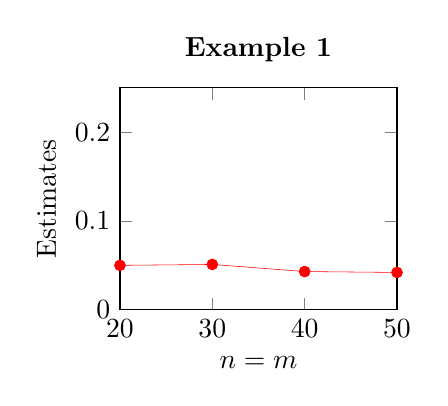
\begin{tikzpicture}
\begin{axis}[xmin = 20, xmax = 50, ymin = 0, ymax = 0.25, xlabel = {$n=m$}, ylabel = {Estimates}, title = {\bf Example 1}]
\addplot[color = red,   mark = *, step = 1cm,very thin]coordinates{(20,0.05)(30,0.051)(40,0.043)(50,0.042)};
\end{axis}
\end{tikzpicture}
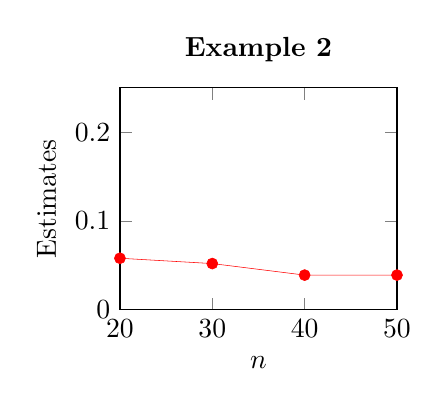
\begin{tikzpicture}
\begin{axis}[xmin = 20, xmax = 50, ymin = 0, ymax = 0.25, xlabel = {$n$}, ylabel = {Estimates}, title = {\bf Example 2}]
\addplot[color = red,   mark = *, step = 1cm,very thin]coordinates{(20,0.058)(30,0.052)(40,0.039)(50,0.039)};

\end{axis}
\end{tikzpicture}
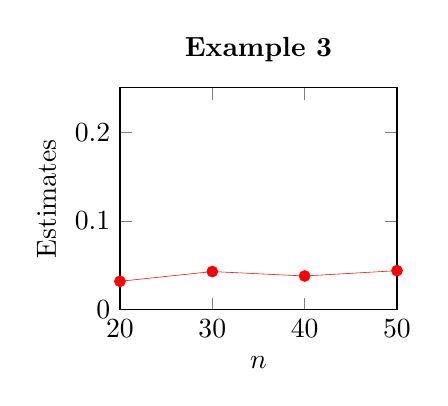
\begin{tikzpicture}
\begin{axis}[xmin = 20, xmax = 50, ymin = 0, ymax = 0.25, xlabel = {$n$}, ylabel = {Estimates}, title = {\bf Example 3}]
\addplot[color = red,   mark = *, step = 1cm,very thin]coordinates{(20,0.032)(30,0.043)(40,0.038)(50,0.044)};
\end{axis}
\end{tikzpicture}
    
    \caption{Results of our test for $n=m=20,30,40$ and $50$ in Examples 1-3.}
    \label{fig:level}
\end{figure}


%\subsection{Simulated power analysis}
%\label{power}
Next, we consider some examples
(Examples 4-7) to compare the power of our test with FAD, WD and BD tests. In each case, we consider 50 observations from each distribution.

\vspace{0.1in}
\noindent
\textbf{Example 4} $X$ is the Wiener process $W$ on $[0,1]$ while $Y$ is distributed as $\mu+W$ and is independent of $X$. We consider two choices of $\mu$, (i) $\mu(t) = r t^2$ and (ii) $\mu(t) = r e^t$, and carry out our experiment for different choices of $r\in \mathbb [0,1]$ as shown in Figure~\ref{fig:5.4} .

\begin{figure}[h!]
\centering
%\begin{tikzpicture}
%\begin{axis}[xmin = 0, xmax = 1, ymin = 0, ymax = 1, xlabel = {$r$}, ylabel = {Estimates}, title = {\bf Example 5.4.(i)}]
%\addplot[mark = *, step = 1cm,very thin]coordinates{(0,0.051)(0.3,0.139)(0.5,0.595)(0.7,0.978)(1,1)};

%\addplot[mark = square*, step = 1cm,very thin]coordinates{(0,0.057)(0.3,0.339)(0.5,0.951)(0.7,0.999)(1,1)};

%\addplot[mark = diamond*, step = 1cm,very thin]coordinates{(0,0.049)(0.3,0.918)(0.5,1)(0.7,1)(1,1)};

%\addplot[mark = triangle*, step = 1cm,very thin]coordinates{(0,0.052)(0.3,0.346)(0.5,0.957)(0.7,1)(1,1)};

%\end{axis}
%\end{tikzpicture}
%\begin{tikzpicture}
%\begin{axis}[xmin = 0, xmax = 1, ymin = 0, ymax = 1, xlabel = {$r$}, ylabel = {Power Estimates}, title = {\bf Example 5.4.(ii)}]
%\addplot[mark = *, step = 1cm,very thin]coordinates{(0,0.051)(0.3,0.134)(0.5,0.643)(0.7,0.991)(1,1)};

%\addplot[mark = square*, step = 1cm,very thin]coordinates{(0,0.057)(0.3,0.388)(0.5,0.99)(0.7,1)(1,1)};

%\addplot[mark = diamond*, step = 1cm,very thin]coordinates{(0,0.049)(0.3,0.984)(0.5,1)(0.7,1)(1,1)};

%\addplot[mark = triangle*, step = 1cm,very thin]coordinates{(0,0.052)(0.3,0.413)(0.5,0.995)(0.7,1)(1,1)};
%\end{axis}
%\end{tikzpicture}

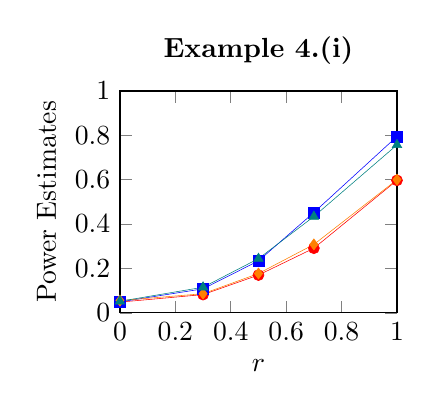
\begin{tikzpicture}
\begin{axis}[xmin = 0, xmax = 1, ymin = 0, ymax = 1, xlabel = {$r$}, ylabel = {Power Estimates}, title = {\bf Example 4.(i)}]
\addplot[color = red, mark = *, step = 1cm,very thin]coordinates{(0,0.048)(0.3,0.082)(0.5,0.17)(0.7,0.291)(1,0.597)};

\addplot[color = blue, mark = square*, step = 1cm,very thin]coordinates{(0,0.049)(0.3,0.108)(0.5,0.234)(0.7,0.452)(1,0.795)};

\addplot[color = orange, mark = diamond*, step = 1cm,very thin]coordinates{(0,0.055)(0.3,0.086)(0.5,0.177)(0.7,0.308)(1,0.6)};

\addplot[color = teal, mark = triangle*, step = 1cm,very thin]coordinates{(0,0.052)(0.3,0.115)(0.5,0.244)(0.7,0.434)(1,0.757)};
\end{axis}
\end{tikzpicture}
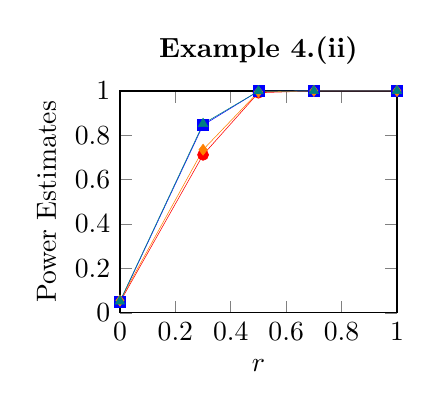
\begin{tikzpicture}
\begin{axis}[xmin = 0, xmax = 1, ymin = 0, ymax = 1, xlabel = {$r$}, ylabel = {Power Estimates}, title = {\bf Example 4.(ii)}]
\addplot[color = red, mark = *, step = 1cm,very thin]coordinates{(0,0.048)(0.3,0.712)(0.5,0.992)(0.7,1)(1,1)};

\addplot[color = blue, mark = square*, step = 1cm,very thin]coordinates{(0,0.049)(0.3,0.846)(0.5,0.999)(0.7,1)(1,1)};

\addplot[color = orange, mark = diamond*, step = 1cm,very thin]coordinates{(0,0.055)(0.3,0.735)(0.5,0.996)(0.7,1)(1,1)};

\addplot[color = teal, mark = triangle*, step = 1cm,very thin]coordinates{(0,0.052)(0.3,0.852)(0.5,0.999)(0.7,1)(1,1)};
\end{axis}
\end{tikzpicture}
    
    \caption{Results of our test (\textcolor{red}{$\bullet$}), FAD test (\textcolor{blue}{$\blacksquare$}), BD test (\textcolor{orange}{$\blacklozenge$}) and WD test (\textcolor{teal}{$\blacktriangle$}) for Example 4.(i) and (ii).}
    \label{fig:5.4}
\end{figure}
\vspace{0.1in}
Here $X$ is pure noise, whereas $Y$ has a non-zero signal $\mu$. The location difference between the  two distributions is an increasing function of $r$. So, as expected, the powers of all tests increased with $r$ (see Figure \ref{fig:5.4}). In these examples, WD and FAD tests performed better. 


\vspace{0.1in}
\noindent
\textbf{Example 5} $X$ and $Y$ are independent random functions as in Example 3 with respective coefficients denoted as $\xi_i^X$ and $\xi_i^Y$ for each $i=1,2,\ldots,9$. Here we consider two scale problems:
(i) $\xi_i^X$s are independent standard normal variables, while $\xi_i^Y$s are mean zero normal random variables with variance $\sigma^2$; (ii) $\xi_i^X$s are independent standard Cauchy variables and $\xi_i^Y$s are the centered Cauchy random variables with scale parameters $\sigma>0$.

\begin{figure}[h!]
\centering
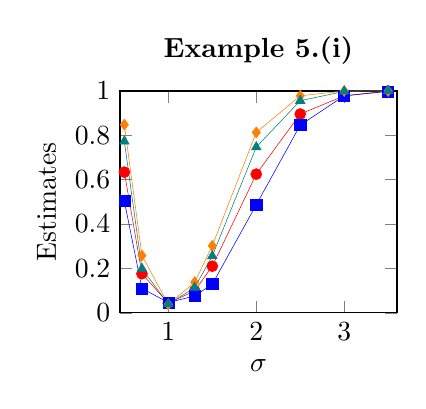
\begin{tikzpicture}
\begin{axis}[xmin = 0.45, xmax = 3.6, ymin = 0, ymax = 1, xlabel = {$\sigma$}, ylabel = {Estimates}, title = {\bf Example 5.(i)}]
\addplot[color = red, mark = *, step = 1cm,very thin]coordinates{(0.5,0.634)(0.7,0.176)(1,0.043)(1.3,0.099)(1.5,0.21)(2,0.625)(2.5,0.896)(3,0.978)(3.5,1)};

\addplot[color = blue, mark = square*, step = 1cm,very thin]coordinates{(0.5,0.503)(0.7,0.11)(1,0.046)(1.3,0.076)(1.5,0.129)(2,0.487)(2.5,0.846)(3,0.978)(3.5,0.998)};

\addplot[color = orange, mark = diamond*, step = 1cm,very thin]coordinates{(0.5,0.848)(0.7,0.258)(1,0.038)(1.3,0.138)(1.5,0.302)(2,0.813)(2.5,0.978)(3,1)(3.5,1)};

\addplot[color = teal, mark = triangle*, step = 1cm,very thin]coordinates{(0.5,0.773)(0.7,0.199)(1,0.039)(1.3,0.114)(1.5,0.256)(2,0.747)(2.5,0.956)(3,0.998)(3.5,1)};

\end{axis}
\end{tikzpicture}
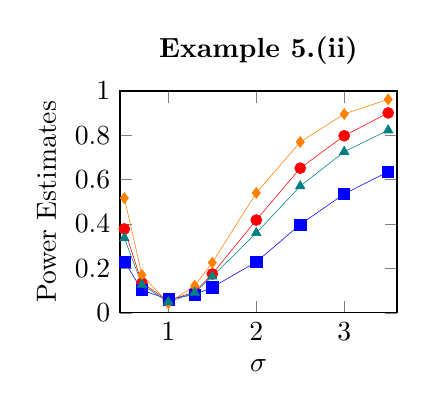
\begin{tikzpicture}
\begin{axis}[xmin = 0.45, xmax = 3.6, ymin = 0, ymax = 1, xlabel = {$\sigma$}, ylabel = {Power Estimates}, title = {\bf Example 5.(ii)}]
\addplot[color = red, mark = *, step = 1cm,very thin]coordinates{(0.5,0.378)(0.7,0.134)(1,0.055)(1.3,0.094)(1.5,0.175)(2,0.418)(2.5,0.652)(3,0.798)(3.5,0.901)};

\addplot[color = blue, mark = square*, step = 1cm,very thin]coordinates{(0.5,0.232)(0.7,0.102)(1,0.061)(1.3,0.082)(1.5,0.115)(2,0.229)(2.5,0.398)(3,0.536)(3.5,0.636)};

\addplot[color = orange, mark = diamond*, step = 1cm,very thin]coordinates{(0.5,0.517)(0.7,0.171)(1,0.043)(1.3,0.122)(1.5,0.226)(2,0.54)(2.5,0.77)(3,0.896)(3.5,0.962)};

\addplot[color = teal, mark = triangle*, step = 1cm,very thin]coordinates{(0.5,0.337)(0.7,0.127)(1,0.048)(1.3,0.091)(1.5,0.164)(2,0.36)(2.5,0.571)(3,0.726)(3.5,0.823)};
\end{axis}
\end{tikzpicture}
  
\caption{Results of our test (\textcolor{red}{$\bullet$}), FAD test (\textcolor{blue}{$\blacksquare$}), BD test (\textcolor{orange}{$\blacklozenge$}) and WD test (\textcolor{teal}{$\blacktriangle$}) for Examples 5 (i) and (ii).}
\label{fig:5.5}
\end{figure}

\vspace{0.1in}
Here, as $\sigma$ deviates from 1, since the scale difference between the two distributions increases, the power of a test is also expected to increase. Figure \ref{fig:5.5} shows the powers of different tests. Here the BD test has the best performance, but our test is competitive with BD test. In 4 (i) the WD test has an edge over our test but in 5.4. (ii) our test outperforms the WD test.

\vspace{0.1in}
\textbf{Example 6} Let $P_{a,b}$ denote the uniform distribution over $S_{a,b} = \big\{(x,y)\in\R\mid a^2<x^2+y^2<b^2\big\}$. We take $X(t) = \xi_1\sin(t)+\xi_2\cos(t), ~t\in[0,1]$ and $Y(t) = \eta_1\sin(t)+\eta_2\cos(t), ~t\in[0,1]$, where $(\xi_1,\xi_2)\sim P_{1,2}$, and $(\eta_1,\eta_2)\sim P_{1,\mu}$ with $\mu>1$.

\vspace{0.1in}
\textbf{Example 7} Let $X(t) = \sum_{i=1}^9 \xi_i^X \psi_i(t)+W(t)$ and $Y(t) = \sum_{i=1}^9 \xi_i^Y \psi_i(t)+ W(t)$, where $W$ is the Wiener process on $[0,1]$, and $\{\psi_i\}$ is the trigonometric basis on $L_2([0,1])$ as in Example 3. We assume $\xi_i^X$s are i.i.d standard Cauchy random variables and $\xi_i^Y$s are independently generated from an equal mixture of two Cauchy distributions with a common scale parameter 1 and locations $0$ and $\mu$, respectively.

\begin{figure}[!h]
\centering
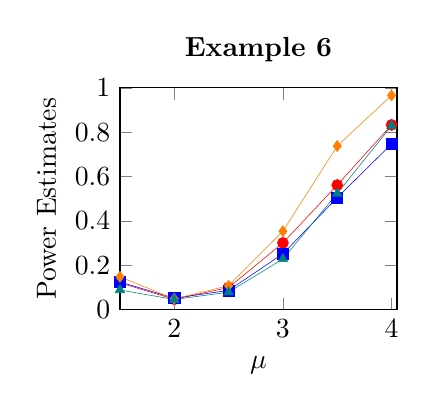
\begin{tikzpicture}
\begin{axis}[xmin = 1.5, xmax = 4.05, ymin = 0, ymax = 1, xlabel = {$\mu$}, ylabel = {Power Estimates}, title = {\bf Example 6}]
\addplot[color = red,mark = *, step = 1cm,very thin]coordinates{(1.5,0.121)(2,0.047)(2.5,0.1)(3,0.301)(3.5,0.562)(4,0.833)(4.5,0.955)(5,0.994)};

\addplot[color = blue, mark = square*, step = 1cm,very thin]coordinates{(1.5,0.125)(2,0.052)(2.5,0.087)(3,0.252)(3.5,0.505)(4,0.747)(4.5,0.895)(5,0.995)};

\addplot[color = orange, mark = diamond*, step = 1cm,very thin]coordinates{(1.5,0.148)(2,0.049)(2.5,0.108)(3,0.354)(3.5,0.738)(4,0.966)(4.5,0.993)(5,1)};

\addplot[color = teal, mark = triangle*, step = 1cm,very thin]coordinates{(1.5,0.089)(2,0.046)(2.5,0.079)(3,0.229)(3.5,0.524)(4,0.829)(4.5,0.965)(5,0.994)};
\end{axis}
\end{tikzpicture}
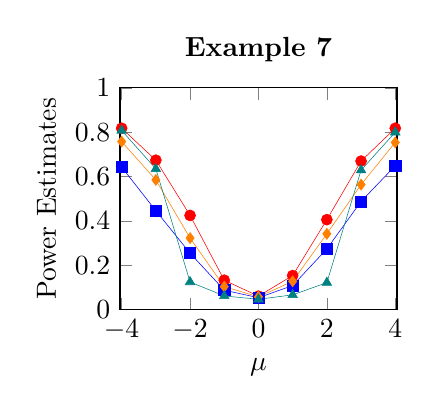
\begin{tikzpicture}
\begin{axis}[xmin = -4.05, xmax = 4.05, ymin = 0, ymax = 1, xlabel = {$\mu$}, ylabel = {Power Estimates}, title = {\bf Example 7}]
\addplot[color = red, mark = *, step = 1cm,very thin]coordinates{(-4,0.818)(-3,0.674)(-2,0.425)(-1,0.133)(0,0.061)(1,0.154)(2,0.406)(3,0.67)(4,0.818)};

\addplot[color = blue, mark = square*, step = 1cm,very thin]coordinates{(-4,0.643)(-3,0.446)(-2,0.255)(-1,0.088)(0,0.054)(1,0.109)(2,0.274)(3,0.488)(4,0.649)};

\addplot[color = orange, mark = diamond*, step = 1cm,very thin]coordinates{(-4,0.758)(-3,0.585)(-2,0.323)(-1,0.104)(0,0.058)(1,0.128)(2,0.342)(3,0.564)(4,0.754)};

\addplot[color = teal, mark = triangle*, step = 1cm,very thin]coordinates{(-4,0.808)(-3,0.635)(-2,0.125)(-1,0.062)(0,0.047)(1,0.067)(2,0.122)(3,0.629)(4,0.8)};
\end{axis}
\end{tikzpicture}
    \caption{Results of our test (\textcolor{red}{$\bullet$}), FAD test (\textcolor{blue}{$\blacksquare$}), BD test (\textcolor{orange}{$\blacklozenge$}) and WD test (\textcolor{teal}{$\blacktriangle$})for Examples 6 and 7.}
    \label{fig:5.6-5.7}
\end{figure}

\vspace{0.1in}
In Example 6, the BD test had the best performance closely followed by our proposed test, but in Example 7, our test outperformed its all competitors (see Figure \ref{fig:5.6-5.7}). In Example 7, the WD test had a competitive  performance for large $\mu$, but for smaller values of $\mu$, it had a very poor performance. 

\subsection{Analysis of DTI data}
\label{real data}

\begin{figure}[!h]
    \centering
    \includegraphics[scale = 0.30]{H_Male.png}
    \includegraphics[scale = 0.30]{H_Female.png}
    \includegraphics[scale = 0.30]{MS_Male.png}
    \includegraphics[scale = 0.30]{MS_Female.png}
    \caption{The FA tract profiles on the first visit, divided according to health status and gender.}
    \label{fig:dti}
\end{figure}

For further evaluation of the performance of our test, we  analyzed the DTI dataset available in the R package `refund'. The MRI/DTI data were collected at Johns Hopkins University and the Kennedy-Krieger Institute. Diffusion tensor imaging (DTI) is a magnetic resonance imaging technology that traces water diffusivity in the brain and helps to create an image of the white matter tract. This dataset has been studied in \cite{dti2011,dti2012} in the context of penalized functional regression. Several measurements of water diffusion are provided by DTI, but here we work with the fractional anisotropy (FA) tract profiles recorded at $93$ different locations of the corpus callosum. The dataset contains measurements on 100 `Multiple Sclerosis patients (MS)' and 42 `healthy controls (HC)'. While the number of visits for the MS patients ranges between 2 and 8, each healthy person visits just once. So, we consider only the FA tract profiles upon the first visit of the subjects. The subject with ID `2017' have some missing values. We delete that observation and work with the remaining 99 MS patients and 42 healthy controls. Among the subjects, there were both males and females. To test whether the `health status' or the `gender' of the subject affects the FA tract profile, we divide the dataset into four groups each corresponding to a particular combination of gender and health status. Figure \ref{fig:dti} displays the FA tracts divided into these four groups. 

Taking one pair of groups at a time, we test for the distributional difference. So, here we consider
consider ${4\choose2} = 6$ cases: (C1) HC males vs. HC females, (C2) HC males vs. MS males, (C3) HC males vs. MS females, (C4) HC females vs. MS males, (C5) HC females vs. MS females and (C6) MS males vs. MS females.  The p-values of our test, BD test, WD test, and Bonferonni corrected p-value of FAD test are reported in Table \ref{tab:pval-table}. The permutation procedure was repeated 10,000 times to calculate the p-values in this scenario. Note that in many cases, the WD test fails to detect the distributional difference when the others reject the null hypothesis at $5\%$ level of significance. Our analysis suggests that the distributional difference among the males and females was statistically insignificant, but the distribution of the FA tract profile differs significantly depending on the health status. 


\begin{table}[h]
    \centering
    \begin{tabular}{ccccc} \hline
    %\toprule
   Case & our test & BD Test & WD Test & FAD Test\\ \hline
    %\midrule
        (C1) & $0.722$ & $0.803$ & $0.369$ & $0.449$\\
        (C2) & $1\times 10^{-4}$ & $1\times 10^{-4}$ & $0.096$ & $7\times 10^{-6}$\\
        (C3) & $1\times 10^{-4}$ & $1\times 10^{-4}$ & $1\times 10^{-4}$ & $8\times10^{-6}$\\
        (C4) & $0.004$ & $0.001$ & $0.221$ & $0.002$\\
        (C5) & $5\times 10^{-4}$ & $4\times 10^{-4}$ & $0.542$ & $5\times 10^{-4}$\\
        (C6) & $0.598$ & $0.638$ & $0.639$ & $0.316$\\ \hline
    %\bottomrule
    \end{tabular}
    \caption{p-values of different our test, BD test, WD test, and Bonferroni corrected p-value of FAD test.}
    \label{tab:pval-table}
\end{table}


\section{Discussion and conclusion}

In this article, we have proposed a two-sample test for functional data, where observations are modelled as elements of separable Hilbert spaces. We have derived the limiting distribution of our proposed test statistic under fixed and contiguous alternatives for kernels with fixed bandwidth and established the consistency of our test even when the data-driven bandwidths are plugged in. However, it is not transparent what happens to the power of the test under contiguous alternatives. If the 
data-driven bandwidth has a sufficiently fast convergence to a non-zero limit, the asymptotic behaviour of the permutation test is expected to be the same as in the case of fixed bandwidth. But it is not clear when we will have such a faster convergence. This can be investigated as an interesting research problem.

 The proposed tests can be generalized to $k$-sample problems as well, where one needs to use the pairwise distance among the kernel mean embedding of the uni-dimensional projections - corresponding to different distributions $F_1, F_2,\ldots, F_k$. The expectation of the average of these pairwise distances can be used as a generalized pMMD measure for the $k$-sample problem. One can also construct a consistent estimate of this measure and develop a $k$-sample test based on it. The large sample behavior of the resulting test can also be investigated using the theory presented in this article. 
\vspace{0.1in}

\textbf{Acknowledgements:} The author is indebted to his advisor Anil K. Ghosh for introducing him to the two sample tests literature and for his guidance, encouragement, and support. The author would also like to thank Bhaswar B. Bhattacharya for his helpful comments and Gina-Maria Pomann and Sujit Ghosh for sharing their R codes implementing the FAD test.

%\section{Appendix}

%% if your bibliography is in bibtex format, uncomment commands:
\bibliographystyle{apalike} % Style BST file (imsart-number.bst or imsart-nameyear.bst)
\bibliography{refs.bib}


%%%%%%%%%%%%%%%%%%%%%%%%%%%%%%%%%%%%%%%%%%%%%%
%% Single Appendix:                         %%
%%%%%%%%%%%%%%%%%%%%%%%%%%%%%%%%%%%%%%%%%%%%%%
\begin{appendix}
\section*{Appendix}%% if no title is needed, leave empty \section*{}.

\begin{lemmaA}
    Let $\{X_n\}$ be a sequence of i.i.d. random variables on the measurable space $(\mathcal{X},\mathcal{A})$ from the distribution $P$. Let $h:\mathcal{X}^2\to \R$ be a measurable function such that $\E_Ph^2(X_1,X_2)$, $\E_Ph^2(X_1,X_1)$ are finite and $\E_P h(x_1, X_2) = 0$ almost surely. %$1=f_0,f_1,f_2,\ldots$ be an orthonormal basis of $L_2(\mathcal{X},\mathcal{A},P)$. 
    Then $\int h(x_1,x_2)d\hat G_P(x_1)d\hat G_P(x_2)$ converges in distribution to $\int h(x_1,x_2)d\mathbb{G}_P(x_1)d\mathbb{G}_P(x_2)$ %& = \sum_{(k_1,k_2)\in\mathbb{N}^2}\langle h,f_{k_1}\times f_{k_2}\rangle \int f_{k_1}(u)d\mathbb{G}_P(u)\int f_{k_2}(v)d\mathbb{G}_P(v),
    as $n$ goes to infinity, where $\hat{G}_P = \sqrt{n}(P_n-P)$ (the empirical process based on $X_1,X_2,\ldots,X_n$) and $\mathbb{G}_P$ is the $P-$Brownian Bridge process. %over a suitable class of functions. % and the equality on the right hand side holds in $L_1$ sense.
    \label{limit-vstat-1}
\end{lemmaA}

\begin{proof}[\bf Proof]  
 Let $1=f_0,f_1,f_2,\ldots$ be an orthonormal basis of $L_2(\mathcal{X},\mathcal{A},P)$. Since, $h\in L_2(\mathcal{X}^2,\mathcal{A}^2,P^2)$ and is degenerate, we can write $h = \sum_{k_1,k_2}\langle h,f_{k_1}\times f_{k_2}\rangle f_{k_1}\times f_{k_2}$ where $k_1,k_2\geq 1$. Define,  $V_n(f):=\int f(x_1,x_2)d\hat{G}_P(x_1)d\hat{G}_P(x_2)$. Then for any $g,h\in L_2(\mathcal{X}^2,\mathcal{A}^2,P^2)$,
  $$\text{cov}(V_n(g),V_n(h)) = \frac{1}{n} \text{cov}(\Tilde{h}(X_1,X_1),\Tilde{g}(X_1,X_1))+\frac{2n(n-1)}{n^2}\int \Tilde{h}(u,v)\Tilde{g}(u,v)dP(u)dP(v),$$ $V_n(h)$ is linear in $h$ and $\E\big\{V_n(h)\big\} = \E\big\{\Tilde{h}(X_1,X_1)\big\},$
  where $\Tilde{h}(u,v) = \int h(t,s)d(\delta_u-P)(t)d(\delta_u-P)(s)$, $\Tilde{g}$ is defined analogously. By the degeneracy of $h$, we have $\Tilde{h}(u,v)=h(u,v)$. Since $\E_Ph^2(X_1,X_2)$ and $\E_Ph^2(X_1,X_1)$ are finite, the partial sum of the series $h_l = \sum_{k_1=1}^l\sum_{k_2=1}^l\langle h,f_{k_1}\times f_{k_2}\rangle f_{k_1}\times f_{k_2}$ converges to $h$ in $L_2(P^2)$. Hence, we get that the series $\sum_{k_1,k_2}\langle h,f_{k_1}\times f_{k_2}\rangle V_n(f_{k_1}\times f_{k_2})$ converges in $L_2(P^n)$ (since $\text{Var}\big(V_n(h-h_l)\big)$ and $|\E V_n(h-h_l)|$ both converges to zero as $l$ diverges to infinity). 
  
  Let $\mathcal{F} = \{f_0,f_1,f_2,\ldots\}$. The elements of $\mathcal{F}$ are two units apart with respect to the $L_2$ metric. Then trivially for any $\epsilon>0$ we have,
  $\lim_{\delta\to 0}\limsup_{n\to\infty}P\Big\{\sup_{d(g,h)<\delta, h,g\in \mathcal{F}}|\hat G(g-h)|>\epsilon\Big\} = 0.$
  Hence, the empirical process $\hat G$ is tight over $\ell^\infty(\mathcal{F})$ and $\mathcal{F}$ is a Donsker's class of functions. Thus the finite-dimensional distributions of the process $\{V_n(f_{k_1}\times f_{k_2})\mid (k_1,k_2)\in \mathbb{N}^2\}$ converges to the corresponding finite-dimensional distributions of the process $\{\int f_{k_1}(u)f_{k_2}(v)d\mathbb{G}_P(u)d\mathbb{G}_P(v)\mid (k_1,k_2)\in \mathbb{N}^2\}$. Then by continuous mapping theorem, $\sum_k\langle h_l,f_{k_1}\times f_{k_2}\rangle V_n(f_{k_1}\times f_{k_2})$ converges in distribution to $\sum_k\langle h_l,f_{k_1}\times f_{k_2}\rangle \int f_{k_1}(u)f_{k_2}(v)d\mathbb{G}_P(u)d\mathbb{G}_P(v) = \int h_l(x_1,x_2)d\mathbb{G}_P(x_1)d\mathbb{G}_P(x_2)$ as $n$ grows to infinity. 
  
  Now note that, $\sup_{i\in \mathbb{N}}\E \big(\int f_i(u) d\mathbb{G}_P(u)\big)^2 = \sup_{i\in \mathbb{N}}\Big\{\int f_i^2(u)\,dP(u)-\big(\int f_i(u)dP(u)\big)^2\Big\} = 1$, by orthonormality of the $f_i$s. Let $[l] := \{1,2,\ldots, l\}$, then for any $l_1<l_2$ we have,
  \begin{equation*}
      \begin{split}
          & \E\big|\int h_{l_1}(x_1,x_2)d\mathbb{G}_P(x_1)d\mathbb{G}_P(x_2)-\int h_{l_2}(x_1,x_2)d\mathbb{G}_P(x_1)d\mathbb{G}_P(x_2)\big|\\ 
       = ~& \E\big|\sum_{(i,j)\in [l_2]^2\setminus [l_1]^2} \langle h, f_{i}\times f_j\rangle \int f_i(u) d\mathbb{G}_P(u)\int f_j(u) d\mathbb{G}_P(u)\big|\\
    \leq ~& \sum_{(i,j)\in [l_2]^2\setminus [l_1]^2} \big|\langle h, f_{i}\times f_j\rangle\big| \E\big|\int f_i(u) d\mathbb{G}_P(u)\int f_j(u) d\mathbb{G}_P(u)\big|\\
    \leq ~& \sum_{(i,j)\in [l_2]^2\setminus [l_1]^2} \big|\langle h, f_{i}\times f_j\rangle\big| \sqrt{\E\big(\int f_i(u) d\mathbb{G}_P(u)\big)^{2}\E\big(\int f_i(u) d\mathbb{G}_P(u)\big)^{2}}\\
    \leq ~& \sum_{(i,j)\in [l_2]^2\setminus [l_1]^2} \big|\langle h, f_{i}\times f_j\rangle\big| \leq \big(\sum_{(i,j)\in [l_2]^2\setminus [l_1]^2} \langle h, f_{i}\times f_j\rangle^2\big)^{1/2}
      \end{split}
  \end{equation*}
  Since $h_l$ converges to $h$ in $L_2(P^2)$, it is also a Cauchy sequence. Hence, for any $\epsilon>0$, we can get an $N\in\mathbb{N}$ such that, $\sum_{(i,j)\in [l_2]^2\setminus [l_1]^2} \langle h, f_{i}\times f_j\rangle^2<\epsilon^2$ for any $l_1,l_2\geq N$ and then we also have,
  $$\E\big|\int h_{l_1}(x_1,x_2)d\mathbb{G}_P(x_1)d\mathbb{G}_P(x_2)-\int h_{l_2}(x_1,x_2)d\mathbb{G}_P(x_1)d\mathbb{G}_P(x_2)\big|<\epsilon.$$
  
  Hence, the sequence $\int h_{l}(x_1,x_2)d\mathbb{G}_P(x_1)d\mathbb{G}_P(x_2)$ is Cauchy in $L_1$. It is easy to see that the limit of this sequence of random variables is $\int h(x_1,x_2)d\mathbb{G}_P(x_1)d\mathbb{G}_P(x_2)$.

  Denote the characteristic function of $\int h_l(u,v)d\hat G(u)d\hat G(v)$ and $\int h(u,v)d\hat G(u)d\hat G(v)$ by $\phi_{nl}(t)$ and $\phi_n(t)$, repectively. Also, let $\phi_l(t)$ and $\phi(t)$ be the characteristic function of $\int h_l(u,v)d\mathbb{G}(u)d\mathbb{G}(v)$ and $\int h(u,v)d\mathbb{G}(u)d\mathbb{G}(v)$, respectively. Then by the previous arguments we can say that for any $\epsilon>0$ and any $t\in\R$, we can find $K\in\mathbb{N}$ such that,
  $|\phi_{l}(t)-\phi(t)|<\epsilon$ for all $l\geq K$. Therefore, it is easy to see that for all $t\in\R$, and for all $l\geq K$, 
  \begin{equation*}
      \begin{split}
          \lim_{n\to\infty}|\phi_{n}(t)-\phi(t)| & \leq \lim_{n\to\infty}|\phi_{nl}(t)-\phi_n(t)|+ \lim_{n\to\infty}|\phi_{nK}(t)-\phi_{K}(t)|+|\phi_l(t)-\phi(t)|\\
          & = \lim_{n\to\infty}|\phi_{nl}(t)-\phi_n(t)|+\epsilon\\
          & \leq |t| \lim_{n\to\infty}\Big\{\E\big\{|\int h_l(u,v)d\hat G(u)d\hat G(v)-\int h(u,v)d\hat G(u)d\hat G(v)|^2\big\}\Big\}^{1/2}+\epsilon\\
          & = |t| \left\{2\E\big\{(h-h_l)^2(X_1,X_2)\big\}+\big\{\E\{(h-h_l)(X_1,X_1)\}\big\}^2\right\}^{1/2}+\epsilon.
      \end{split}
  \end{equation*}
  In the second last inequality we have used the fact that $\E\{|e^{itX}-1|\}\leq |t|\E|X|\leq |t|\{\E|X|^2\}^{1/2}$.  Now as $l$ grows to infinity we have $\lim\limits_{n\to\infty}|\phi_{n}(t)-\phi(t)|<\epsilon$ and as $\epsilon$ is arbitrary we can say $\lim\limits_{n\to\infty}|\phi_{n}(t)-\phi(t)|=0$. Hence, $\int h(u,v)d\hat G(u)d\hat G(v)$ converges in distribution to $\int h(u,v)d\mathbb{G}(u)d\mathbb{G}(v)$.  
  %the result follows immediately by showing that the corresponding characteristic functions converge. 
\end{proof}

\begin{lemmaA}
    Let $\{X_n\}$ and $\{Y_m\}$ be two independent sequences of i.i.d. random variables on the measurable space $(\mathcal{X},\mathcal{A})$ from distributions $P$ and $Q$ respectively. Let $h:\mathcal{X}^2\to \R$ be a measurable function such that $\E_Ph^2(X_1,Y_1)<\infty$, which is not necessarily symmetric. Assume $\E_P h(x_1, Y_1) = 0$ and $\E_P h(X_1, y_1) = 0$ almost surely. %Let $1=f_0,f_1,f_2,\ldots$ be an orthonormal basis of $L_2(\mathcal{X},\mathcal{A},P)$ and $1=g_0,g_1,g_2,\ldots$ be an orthonormal basis of $L_2(\mathcal{X},\mathcal{A},P)$. 
    Then,
    $\sqrt{nm}\int h(x_1,y_1)d\hat{G}_P(x_1)d\hat{G}_Q(y_1)$ converges in distribution to $\int h(x_1,y_1)d\mathbb{G}_P(x_1)d\mathbb{G}_Q(y_1),$ as $\min\{n,m\}$ goes to infinity, where $\hat{G}_P = \sqrt{n}(P_n-P)$ and $\hat{G}_Q=\sqrt{m}(Q_m-Q)$ are the empirical processes based on the observations $X_1,X_2,\ldots,X_n$ and $Y_1,Y_2,\ldots,Y_m$ respectively, and $\mathbb{G}_P$ and $\mathbb{G}_Q$ are independent Brownian Bridge processes.% over a suitable class of functions. %$\mathcal{F}$ containing the basis $\{f_0,f_1,f_2,\ldots\}\cup\{g_0,g_1,g_2,\ldots\}$.% and the stochastic integral on the right hand side is defined in $L_1$ sense as in Lemma A.\ref{limit-vstat-1}.
    \label{limit-vstat-2}
\end{lemmaA}

\begin{proof}[\bf Proof]
    Let $1=f_0,f_1,f_2,\ldots$ be an orthonormal basis of $L_2(\mathcal{X},\mathcal{A},P)$ and $1=g_0,g_1,g_2,\ldots$ be an orthonormal basis of $L_2(\mathcal{X},\mathcal{A},Q)$. Define, $\mathcal{F}=\{f_0,f_1,f_2,\ldots\}\cup\{g_0,g_1,g_2,\ldots\}$. Using similar argument as in Lemma A.\ref{limit-vstat-1} we can argue that $\mathcal{F}$ is a Donsker's class of functions.
    
    Let us define, $T_n(f) := \sqrt{nm}\int h(x_1,y_1)d\hat{G}_P(x_1)d\hat{G}_Q(y_1)$. Then for $g,h\in L_2(\mathcal{X}^2,\mathcal{A}^2,P\otimes Q)$, $\text{cov}(T_n(g),T_n(h)) = \int \Tilde{g}(u,v)\Tilde{h}(u,v)dP(u)dQ(v),$ and $\E\big\{T_n(h)\big\} = \E\big\{\Tilde{h}(X_1,Y_1)\big\} = 0,$
    where $\Tilde{h},\Tilde{g}$ are defined as in Lemma A.\ref{limit-vstat-1}. Now write $h$ as a series $\sum_{k_1,k_2}\langle h, f_{k_1}\times g_{k_2}\rangle f_{k_1}\times g_{k_2}$ where $k_1,k_2\geq 1$ (by the degeneracy assumption). Since, $h_l = \sum_{(k_1,k_2)\in [l]^2}\langle h, f_{k_1}\times g_{k_2}\rangle f_{k_1}\times g_{k_2}$ converges to $h$ in $L_2(P\otimes Q)$, we have $T_n(h_l)$ converges to $T_n(h)$ in $L_2(P^n\otimes Q^m)$(as $\text{Var}\big(h-h_l\big)$ converges to zero as $l$ goes to infinity). 
    
    Since $\mathcal{F}$ is a class of Donsker's function, the finite-dimensional distributions of the process $\{T_n(f_{k_1}\times g_{k_2})\mid (k_1,k_2)\in \mathbb{N}^2\}$ converges to the corresponding finite-dimensional distributions of the process $\{\int f_{k_1}(u)g_{k_2}(v)d\mathbb{G}_P(u)d\mathbb{G}_Q(v)\mid (k_1,k_2)\in \mathbb{N}^2\}$. Then $\sum_k\langle h_l,f_{k_1}\times g_{k_2}\rangle T_n(f_{k_1}\times g_{k_2})$ converges in distribution to $\sum_k\langle h_l,f_{k_1}\times g_{k_2}\rangle \int f_{k_1}(u)g_{k_2}(v)d\mathbb{G}_P(u)d\mathbb{G}_Q(v) = \int h_l(x_1,x_2)d\mathbb{G}_P(x_1)d\mathbb{G}_Q(x_2)$ as $\min\{n,m\}$ grows to infinity, by continuous mapping theorem. 
    
    Now, $\E \big|\int f_i(u) d\mathbb{G}_P(u)\big| = \sqrt{2/\pi}\big(\int f_i^2(u)dP(u)\big)^{1/2} = \sqrt{2/\pi}~\forall i$, by orthonormality of the basis elements. Similarly, $\E \big|\int f_i(u) d\mathbb{G}_P(u)\big| = \sqrt{2/\pi}~\forall i$. Then for any $l_1<l_2$ we have, 
    \begin{equation*}
      \begin{split}
          & \E\big|\int h_{l_1}(x_1,x_2)d\mathbb{G}_P(x_1)d\mathbb{G}_Q(x_2)-\int h_{l_2}(x_1,x_2)d\mathbb{G}_P(x_1)d\mathbb{G}_Q(x_2)\big|\\ 
       = ~& \E\big|\sum_{(i,j)\in [l_2]^2\setminus [l_1]^2} \langle h, f_{i}\times g_j\rangle \int f_i(u) d\mathbb{G}_P(u)\int g_j(u) d\mathbb{G}_Q(u)\big|\\
    \leq ~& \sum_{(i,j)\in [l_2]^2\setminus [l_1]^2} \big|\langle h, f_{i}\times g_j\rangle\big| \E\big|\int f_i(u) d\mathbb{G}_P(u)\int g_j(u) d\mathbb{G}_Q(u)\big|\\
    = ~& \sum_{(i,j)\in [l_2]^2\setminus [l_1]^2} \big|\langle h, f_{i}\times g_j\rangle\big|~\E\big|\int f_i(u) d\mathbb{G}_P(u)\big|~\E\big|\int g_j(u) d\mathbb{G}_Q(u)\big| \\
    \leq ~& \sum_{(i,j)\in [l_2]^2\setminus [l_1]^2} \big|\langle h, f_{i}\times f_j\rangle\big|\frac{2}{\pi} \leq \frac{2}{\pi}\Big(\sum_{(i,j)\in [l_2]^2\setminus [l_1]^2} \big|\langle h, f_{i}\times f_j\rangle\big|^2\Big)^{1/2}.
      \end{split}
  \end{equation*}
    Now using similar arguments as in Lemma A.\ref{limit-vstat-1} gives us our result. 
\end{proof}

\begin{proof}[\bf Proof of Theorem \ref{thm1}]
Let $X\sim F$ and $Y\sim G$ and define $\phi:\H\to {\mathbb C}$ as
$\phi(f) = \E\{e^{i\langle X,f \rangle}\}-\E\{e^{i\langle Y,f \rangle}\}.$
Notice that the function $\phi$ is continuous and $\phi(f)  = 0~ \forall f\in\H$ implies the two distributions $F$ and $G$ are equal. It is easy to see that if $F=G$, $T(F^f,G^f)=0$ for any $f\in\H$. Hence, when $F=G$, $\zeta^\nu(F,G)=0$ for any probability distribution $\nu$ on $\H$ follows trivially. Now  $\zeta^\nu(F,G) = 0$ implies there exists a Borel measurable set $E\in\mathcal{B}(\H)$ such that $\nu(E) = 1$ and $T(F^f,G^f) = 0~ \forall f\in E$. Hence, by the assumption on $T$, we have
$\phi(f) = 0 ~\forall f\in E$. Thus when $supp\{\nu\}$ is contains the surface of the unit sphere, it follows that for any $f\in\H$, $\langle X,f\rangle = \|f\|\langle X,f/\|f\|\rangle$ and $\langle Y,f\rangle = \|f\|\langle Y,f/\|f\|\rangle$ have the same distribution. Hence, we have $\phi(f) = 0~\forall f\in\H$. 
\end{proof}


\begin{proof}[\bf Proof of Theorem \ref{thm2}]
Let us first consider the following claim.

\textbf{Claim:} Suppose that $X$ is a random variable of a Hilbert space $\H$ with distribution $F$. If $supp\{F\}\subset \H_0$ where $\H_0$ is a closed subspace of $\H$, then $X$ and $QX$ have the same distribution
, where $Q:\H \rightarrow \H_0$ is the projection operator onto $\H_0$.

The claim can be proven by showing that the the characteristic function of $X$ and $QX$ are identical. Now take any arbitrary $\theta \in\H$, and note that
\begin{equation*}
    \begin{split}
        \E\{e^{i\langle X,\theta \rangle}\}  =& \int_\H e^{i\langle x,\theta\rangle} \,dF(x)
         = \int_{\H_0} e^{i\langle x,\theta\rangle} \,dF(x)
         = \int_{\H_0} e^{i\langle Qx,Q\theta\rangle+i\langle (I-Q)x,(I-Q)\theta\rangle}\,dF(x)\\
         & = \int_{\H_0} e^{i\langle Qx,Q\theta\rangle+i\langle 0,(I-Q)\theta\rangle}\,dF(x)
         = \int_{\H_0} e^{i\langle Qx,\theta\rangle}\,dF(x) = \E\{e^{i\langle QX,\theta \rangle}\}.
    \end{split}
\end{equation*}

Hence the claim holds. Denote $\H_0 = \overline{span\{supp\{F\}\cup supp\{G\}\}}$, clearly $\H_0$ is a closed subspace of $\H$. Let $Q$ denote the projection operator from $\H$ to $\H_0$. Then 
\begin{equation*}
    \begin{split}
     \phi(f)  &= \E\{e^{i\langle X,f \rangle}\}-\E\{e^{i\langle Y,f \rangle}\}
         = \int_{\H}e^{i\langle x,f \rangle}dF(x) - \int_{\H}e^{i\langle y,f \rangle}dG(y)\\
        & = \int_{\H_0}e^{i \langle x,f \rangle}dF(x) - \int_{\H_0}e^{i \langle y,f \rangle}dG(y)\\
        & = \int_{\H_0}e^{i \langle Qx,Qf \rangle+i \langle (I-Q)x,(I-Q)f \rangle}dF(x) - \int_{\H_0}e^{i\langle Qy,Qf \rangle+i \langle (I-Q)y,(I-Q)f \rangle}dG(y)\\
        & = \int_{\H_0}e^{i \langle Qx,Qf \rangle}dF(x) - \int_{\H_0}e^{i\langle Qy,Qf \rangle}dG(y)\\
        & {=} \int_{\H_0}e^{i \langle x,Qf \rangle}dF(x) - \int_{\H_0}e^{i \langle y,Qf \rangle}dG(y)~~~~~~~~~\mbox{ (Using Claim with $\theta = Qf$) }\\
        & = \phi(Qf)
    \end{split}
\end{equation*}

This shows that it is enough to consider the value of $\phi(.)$ on $\H_0$. Now if $\zeta^{(F+G)/2}(F,G) = 0$, we have $\phi(f) = 0$ for all $f\in supp\{F\}\cup supp\{G\}$. So, $\langle X, f\rangle$ and $\langle Y, f\rangle$ are independent and identically distributed for any fixed $f\in supp\{F\}\cup supp\{G\}$. Now for any $g\in\H_0$ we can write $g = \sum_{i=1}^\infty a_{i} f_{i}$ for $\{f_{i}\}\subset supp\{F\}\cup supp\{G\}$ and $\{a_{i}\}\subset \R$. It follows trivially that $\langle X,g\rangle = \sum_{i=1}^\infty a_{i}\langle X, f_{i}\rangle$ and $\langle Y,g\rangle = \sum_{i=1}^\infty a_{i}\langle Y, f_{i}\rangle$ are also independent and identically distributed. This implies $\phi(g)= 0 ~\forall g\in\H_0$ and by Claim 1 and 2 $\phi(g) = 0~ \forall g\in\H$. So, if $\zeta^{(F+G)/2}(F,G) = 0$, $X$ and $Y$ are identically distributed. 
\end{proof}

\noindent
\begin{proof}[\bf Proof of Proposition \ref{depprop}]
\text{  }
\begin{itemize}
    \item[(a)] It is easy to see that,
    \begin{equation*}
        \begin{split}
            \E\{g(X_1,X_2,X_3;Y_1,Y_2,Y_3)\} & = \frac{1}{2}\int MMD(F^f,G^f)dF(f)+\frac{1}{2}\int MMD(F^f,G^f)dG(f)\\
            & = \frac{1}{2}\int MMD(F^f,G^f)d(F+G)(f)\\
            & = \zeta^{(F+G)/2}(F,G) = \zeta(F,G).
        \end{split}
    \end{equation*}
    \item[(b)] The proof of this statement follows from Theorem \ref{thm2}.
    \item[(c)] Note, if $U:\mathcal{H}\to\mathcal{G}$ is a unitary operator ($U$ is a linear bijective map with $\langle Ux,Uy\rangle = \langle x,y\rangle$), then $g(.)$ remains invariant of this operation, i.e., 
    $$g(UX_1,UX_2,UX_3;UY_1,UY_2,UY_3) = g(X_1,X_2,X_3;Y_1,Y_2,Y_3).$$
    
    Thus $\zeta(F,G) = \E\{g(X_1,X_2,X_3;Y_1,Y_2,Y_3)\} = \E\{g(UX_1,UX_2,UX_3;UY_1,UY_2,UY_3)\} = \zeta(F\circ U^{-1}, G\circ U^{-1})$. Thus $\zeta$ is invariant under unitary operations.
    
    \item[(d)] This follows by simply applying the Dominated Convergence Theorem.
\end{itemize}
\end{proof}




\begin{proof}[\bf Proof of Theorem \ref{largesampleres}]

First let us note that $\zeta(F,G) = \E\{g^*(X_1,X_2,X_3;Y_1,Y_2,Y_3)\}$ and define the function, $\varphi:\R^2\to\R$ as $\varphi(t,s) = \zeta(F+t\sqrt{n}(F_n-F),G+s\sqrt{m}(G_m-G))$, where $F_n$ and $G_m$ are the empirical probability distribution based on the observed data $\mathcal{X}$ and $\mathcal{Y}$. Clearly, $\varphi$ is a bivariate polynomial with random coefficients. It is easy to see that the coefficients are tight (by Lemma A.\ref{limit-vstat-1} and A.\ref{limit-vstat-2}). Also note that $\hat\zeta_{n,m} = \varphi(1/\sqrt{n},1/\sqrt{m})$ and $\varphi(0,0) = \zeta(F,G)$. Hence the limiting distribution of $\hat\zeta_{n,m}$ will be determined by the leading non-zero coefficient of $\varphi(1/\sqrt{n},1/\sqrt{m})$. Now, for any $n,m\in\mathbb{N}$,
$$\varphi(1/\sqrt{n},1/\sqrt{m}) = \varphi(0,0)+\frac{1}{\sqrt{n}}\frac{\partial}{\partial t}\varphi(t,s)\Big|_{(0,0)}+\frac{1}{\sqrt{m}}\frac{\partial}{\partial s}\varphi(t,s)\Big|_{(0,0)}+R_{n,m},$$

where $R_{n,m}$ is of stochastic order $O_P\big(\{1/\sqrt{n}+1/\sqrt{m}\}^2\big)$. Note that, 
$$\frac{\partial}{\partial t}\varphi(t,s)\Big|_{(0,0)} = \sqrt{n}\int h_1^*(x)d(F_n-F)(x)\hspace{15pt}\text{ and }\hspace{15pt}\frac{\partial}{\partial s}\varphi(t,s)\Big|_{(0,0)} = \sqrt{m}\int h_2^*(y)d(G_m-G)(y),$$
where $h_1^*(x) = 3~\E\{g^*(x,X_2,X_3;Y_1,Y_2,Y_3)\}$ and $h_2^*(y) = 3~\E\{g^*(X_1,X_2,X_3;y,Y_2,Y_3)\}$, the first order projection of the symmetrized core function $g^*$ upto a constant term. Hence, we have,
$$\hat \zeta_{n,m}-\zeta(F,G) = \frac{1}{\sqrt{n}}\int h_1^*(x)\sqrt{n}d(F_n-F)(x)+\frac{1}{\sqrt{m}}\int h_2^*(y)\sqrt{m}d(G_m-G)(y)+O_{P}\Big(\big\{\frac{1}{\sqrt{n}}+\frac{1}{\sqrt{m}}\big\}^2\Big).$$

Since, $\mathcal{X}$ and $\mathcal{Y}$ are independently generated, the corresponding empirical processes $\sqrt{n}(F_n-F)$ and $\sqrt{m}(G_m-G)$ are also independent of each other. Now if atleast one $h_1^*$ and $h_2^*$ is a non-zero function, applying CLT we have, $\sqrt{nm/n+m}\big\{\hat \zeta_{n,m}-\zeta(F,G)\big\}$ converges in distribution to a normal limiting distribution with mean zero and variance $\lambda \text{Var}\big(h_1^*(X_1)\big)+(1-\lambda)\text{Var}\big(h_2^*(Y_1)\big)$.

If $h_1^*$ and $h_2^*$ are both zero functions, the limiting distribution of $\hat\zeta_{n,m}$ will be determined by coefficients of the higher order terms in the random bivariate polynomial $\varphi(t,s)$. Generally, in such situations, one may have,
$$\zeta_{n,m}-\zeta(F,G) = \frac{1}{2n}\frac{\partial^2}{\partial t^2}\varphi(t,s)\Big|_{(0,0)}+\frac{1}{2m}\frac{\partial^2}{\partial s^2}\varphi(t,s)\Big|_{(0,0)}+\frac{1}{\sqrt{nm}}\frac{\partial^2}{\partial t\partial s}\varphi(t,s)\Big|_{(0,0)} + R_{n,m}.$$

Where $$\frac{\partial^2}{\partial t^2}\varphi(t,s)\Big|_{(0,0)} = n\int h_1^*(u,v)d(F_n-F)(u)d(F_n-F)(v),$$ 
$$\frac{\partial^2}{\partial t\partial s}\varphi(t,s)\Big|_{(0,0)} = \sqrt{nm}\int h_2^*(u,v)d(F_n-F)(u)d(G_m-F)(v),$$
and $$\frac{\partial^2}{\partial s^2}\varphi(t,s)\Big|_{(0,0)} = m\int h_3^*(u,v)d(G_m-F)(u)d(G_m-F)(v),$$
where $h_1^*(u,v), h_2^*(u,v)$ and $h_3^*(u,v)$ are the second order projections of the symmetrized core function $g^*$ upto a constant factor and $R_{n,m} = O_P\big(\{1/\sqrt{n}+1/\sqrt{m}\}^3\big)$. Here the limiting distribution of $nm/(n+m)\big\{\hat \zeta_{n,m}-\zeta(F,G)\big\}$ will depend on the limiting distribution of the random vector $(\frac{\partial^2}{\partial t^2}\varphi(t,s)\Big|_{(0,0)},\frac{\partial^2}{\partial s^2}\varphi(t,s)\Big|_{(0,0)},\frac{\partial^2}{\partial t\partial s}\varphi(t,s)\Big|_{(0,0)})$. Now we prove our result below.

\begin{enumerate}
    \item[(a)] First we will find the functions $h_1^*(x)$ and $h_2^*(y)$ upto an additive constant term. Since adding a constant to the functions does not change the limiting distribution of the empirical stochastic integrals. Note that,
    \begin{equation*}
        \begin{split}
                h_1^*(x) & =3~\E\big\{g^*(x,X_2,X_3;Y_1,Y_2,Y_3)\big\}\\
                & = \Big\{\E\big(g(x,X_2,X_3;Y_1,Y_2,Y_3)+g(X_1,X_2,x;Y_1,Y_2,Y_3)+g(X_1,X_2,x;Y_1,Y_2,Y_3)\big)\Big\},
        \end{split}
    \end{equation*}
    where $g(x_1,x_2,x_3;y_1,y_2,y_3)$ is the function defined in Proposition \ref{depprop} (a). Now,
    \begin{equation*}
    \begin{split}
        & \E\big(g(x,X_2,X_3;Y_1,Y_2,Y_3)\big)\\
        & =  \frac{1}{2}\E\Big\{k\big(\langle X_2,x\rangle, \langle X_3,x\rangle\big)+k\big(\langle Y_2,x\rangle, \langle Y_3,x\rangle\big)
         - 2~k\big(\langle X_2,x\rangle, \langle Y_1,x\rangle\big)\\
         & \hspace{40pt}-2~k\big(\langle x,Y_1\rangle, \langle Y_2, Y_1\rangle\big)\Big\}+c_1,\\
        & \E\big(g(X_1,x,X_3;Y_1,Y_2,Y_3)\big)\\
        & =\frac{1}{2}\E\Big\{k\big(\langle x,X_1\rangle, \langle X_3,X_1\rangle\big)-2~k\big(\langle x,X_1\rangle, \langle Y_1,X_1\rangle\big)
         +k\big(\langle x,Y_1\rangle, \langle X_3,Y_1\rangle\big)\Big\}+c_2,\\
        & \text{and}\\ 
        & \E\big(g(x,X_2,X_3;Y_1,Y_2,Y_3)\big) =  \frac{1}{2}\E\Big\{k\big(\langle X_2,X_1\rangle, \langle x,X_1\rangle\big)+k\big(\langle X_2,Y_1\rangle, \langle x,Y_1\rangle\big)\Big\}+c_3,
    \end{split}
    \end{equation*}
     where $c_1,c_2$ and $c_3$ are constants that depend on he kernel $k(.,.)$ and the distributions $F$ and $G$. Clearly,
     \begin{equation*}
        \begin{split}
            h_1^*(x)~ = & \Big[\E\Big\{k\big(\langle x,X_1\rangle, \langle X_3,X_1\rangle\big)+k\big(\langle X_2,Y_1\rangle, \langle x,Y_1\rangle\big)\\
            & \hspace{20pt}-k\big(\langle x,X_1\rangle, \langle Y_1,X_1\rangle\big)-k\big(\langle x,Y_1\rangle, \langle Y_2, Y_1\rangle\big)\Big\}\Big]+\frac{1}{2}MMD(F^x,G^x)+c.
        \end{split} 
     \end{equation*}
     Under $H_0$, $h_1^*$ is the zero function and under $H_1$, it is non-zero. We can conclude the same for $h_2(y)$ due to structural symmetry of $g$. Hence, $\sqrt{nm/(n+m)}\big(\hat\zeta_{n,m}-\zeta(F,G)\big)$ converges in distribution to $\sqrt{1-\lambda}\int h_1^*(x)d\mathbb{G}_F(x)+\sqrt{\lambda}\int h_2^*(y)d\mathbb{G}_G(y)$ as $\min\{n,m\}$ goes to infinity with $n/(n+m)\to\lambda\in[0,1]$, where $\mathbb{G}_F$ and $\mathbb{G}_G$ are two independent Brownian Bridge processes. The random variable $\sqrt{1-\lambda}\int h_1^*(x)d\mathbb{G}_F(x)+\sqrt{\lambda}\int h_2^*(y)d\mathbb{G}_G(y)$ is a normal random variable with zero mean and variance $(1-\lambda)\text{Var}\big(h_1^*(X)\big)+\lambda)\text{Var}\big(h_2^*(Y)\big)$.
     
    \item[(b)] Here also we will find the functions $h_1^*(u,v),h_2^*(u,v)$ and $h_3^*(u,v)$ upto an additive constant. Since, for any $g$, $\Tilde{(g+c)}(u,v) = g(u,v)+c-\E h(u,V)-c-\E h(U,v)-c+\E h(U,V)+c = \Tilde{g}$ for any constant $c$, as before, here also the additive constant will not effect the limiting distribution of the empirical stochastic integrals. Note that,
    \begin{equation*}
        \begin{split}
            h_1^*(u,v) ~= \Big\{&\E g\big(u,v,X_3;Y_1,Y_2,Y_3\big)+ \E g\big(u,X_2,v;Y_1,Y_2,Y_3\big)+ \E g\big(X_1,u,v;Y_1,Y_2,Y_3\big)\\
            & + \E g\big(v,u,X_3;Y_1,Y_2,Y_3\big)+\E g\big(v,X_2,u;Y_1,Y_2,Y_3\big)+\E g\big(X_1,u,v;Y_1,Y_2,Y_3\big)\Big\}\\
            =: ~~& \Big\{T_1(u,v)+T_2(u,v)\Big\},
        \end{split}
    \end{equation*}
    where $T_1(u,v) = \E g\big(u,v,X_3;Y_1,Y_2,Y_3\big)+ \E g\big(u,X_2,v;Y_1,Y_2,Y_3\big)+ \E g\big(X_1,u,v;Y_1,Y_2,Y_3\big)$ and $T_1$ and $T_2$ are related as in $T_2(u,v) = T_1(v,u)$. Hence, it is enough to find $T_1(u,v)$. Now,
    \begin{equation*}
    \begin{split}
        & \E\big(g(u,v,X_3;Y_1,Y_2,Y_3)\big) \\
        & =~ \frac{1}{2}\E\Big\{k\big(\langle v,u\rangle, \langle X_3,u\rangle\big)+k\big(\langle Y_2,u\rangle, \langle Y_3,u\rangle\big)- 2~k\big(\langle v,u\rangle, \langle Y_1,u\rangle\big)\\
        &~~~+k\big(\langle v,Y_1\rangle, \langle X_3, Y_1\rangle\big)+k\big(\langle Y_2,Y_1\rangle, \langle Y_3, Y_1\rangle\big)-2~k\big(\langle u,Y_1\rangle, \langle Y_2, Y_1\rangle\big)\Big\},\\
        & \E\big(g(u,X_2,v;Y_1,Y_2,Y_3)\big)\\
        & =~ \frac{1}{2}\E\Big\{k\big(\langle X_2,u\rangle, \langle v,u\rangle\big)+k\big(\langle Y_2,u\rangle, \langle Y_3, u\rangle\big)-2~k\big(\langle X_2,u\rangle, \langle Y_1,u\rangle\big)\\
        & ~~~+k\big(\langle X_2,Y_1\rangle, \langle v,Y_1\rangle\big)+k\big(\langle Y_2,Y_1\rangle, \langle Y_3, Y_1\rangle\big)-2~k\big(\langle u,Y_1\rangle, \langle Y_2, Y_1\rangle\big)\Big\},\\
    \end{split}
    \end{equation*}
    and
    \begin{equation*}
        \begin{split}
            & \E\big(g(X_1,u,v;Y_1,Y_2,Y_3)\big)\\
            & =~ \frac{1}{2}\E\Big\{k\big(\langle u,X_1\rangle, \langle v,X_1\rangle\big)+k\big(\langle Y_2,X_1\rangle, \langle Y_3,X_1\rangle\big)-2~k\big(\langle u,X_1\rangle, \langle Y_1,X_1\rangle\big)\\
            & ~~~+k\big(\langle u,Y_1\rangle, \langle v, Y_1\rangle\big)+k\big(\langle Y_2,Y_1\rangle, \langle Y_3, Y_1\rangle\big)-2~k\big(\langle X_1,Y_1\rangle, \langle Y_2, Y_1\rangle\big)\Big\}.
        \end{split}
    \end{equation*}
    Therefore, under $H_0$,
    \begin{equation*}
        \begin{split}
            T_1(u,v) ~= & \E\Big\{k\big(\langle v,Y_1\rangle, \langle X_3, Y_1\rangle\big)\Big\}-\E\Big\{k\big(\langle u,X_1\rangle, \langle Y_1, X_1\rangle\big)\Big\}\\
            &-2~\E\Big\{k\big(\langle u,Y_1\rangle, \langle Y_2, Y_1\rangle\big)\Big\}+\E\Big\{k\big(\langle u,Y_1\rangle, \langle v, Y_1\rangle\big)\Big\}+b_1,
        \end{split}
    \end{equation*}
    for some constant $b_1$ depending on the kernel $k(.,.)$ and the distribution $F$ under $H_0$. Similarly we get,
    \begin{equation*}
        \begin{split}
            T_2(u,v) ~= & \E\Big\{k\big(\langle u,Y_1\rangle, \langle X_3, Y_1\rangle\big)\Big\}-\E\Big\{k\big(\langle v,X_1\rangle, \langle Y_1, X_1\rangle\big)\Big\}\\
            &-2~\E\Big\{k\big(\langle v,Y_1\rangle, \langle Y_2, Y_1\rangle\big)\Big\}+\E\Big\{k\big(\langle v,Y_1\rangle, \langle u, Y_1\rangle\big)\Big\}+b_1,
        \end{split}
    \end{equation*}
    for some constant $b_1$ depending on the kernel $k(.,.)$ and the distribution $F$ under $H_0$. Hence we obtain, under $H_0$,
    \begin{equation*}
        \begin{split}
            h_1^*(u,v) = 2\left\{\E\Big\{k\big(\langle u,Y_1\rangle, \langle v, Y_1\rangle\big)\Big\}-\E\Big\{k\big(\langle u,Y_1\rangle, \langle Y_2, Y_1\rangle\big)\Big\}-\E\Big\{k\big(\langle v,Y_1\rangle, \langle Y_2, Y_1\rangle\big)\Big\}\right\}+b_1^*.
        \end{split}
    \end{equation*}
    Clearly, this is symmetric and non-zero. By the structural symmetry of $g$ we also have $h_3^*(u,v)= h_1^*(u,v)$. Also note that,
    \begin{equation*}
        \begin{split}
            h_2^*(u,v) ~= \Big\{&\E g\big(u,X_2,X_3;v,Y_2,Y_3\big)+ \E g\big(u,X_2,X_3;Y_1,v,Y_3\big)+ \E g\big(u,X_2,X_3;Y_1,Y_2,v\big)\\
            & + \E g\big(X_1,u,X_3;v,Y_2,Y_3\big)+ \E g\big(X_1,u,X_3;Y_1,v,Y_3\big)+ \E g\big(X_1,u,X_3;Y_1,Y_2,v\big)\\
            & + \E g\big(X_1,X_2,u;v,Y_2,Y_3\big)+ \E g\big(X_1,X_2,u;Y_1,v,Y_3\big)+ \E g\big(X_1,X_2,u;Y_1,Y_2,v\big)\Big\}.
        \end{split}
    \end{equation*}

   Upon simplification, this yields that under $H_0$, 
    $$h_2^*(u,v) = 2\left\{\E\Big\{k\big(\langle u,Y_1\rangle, \langle Y_2, Y_1\rangle\big)\Big\}+\E\Big\{k\big(\langle v,Y_1\rangle, \langle Y_2, Y_1\rangle\big)\Big\}-\E\Big\{k\big(\langle u,Y_1\rangle, \langle v, Y_1\rangle\big)\Big\}\right\}+b_3^*.$$

    Hence, under $H_0$, $h_1^*(u,v) = h_3^*(u,v) = 2~h(u,v)$ (say), then $h_2^*(u,v) = - 2 h(u,v)$ which is a non-zero function. Thus, the limiting distribution of $\hat\zeta_{n,m}$ is determined by the joint asymptotic distribution of $\big(\int h(u,v)d\hat{\mathbb{G}}_F(u)d\hat{\mathbb{G}}_F(v),\int h(u,v)d\hat{\mathbb{G}}_F(u)d\hat{\mathbb{G}}^\prime_F(v),\int h(u,v)d\hat{\mathbb{G}}^\prime_F(u)d\hat{\mathbb{G}}^\prime_F(v)\big)$ where $\hat{\mathbb{G}}_F = \sqrt{n}(\hat F_n-F)$ and $\hat{\mathbb{G}}^\prime_F = \sqrt{m}(\hat G_m-F)$. For joint convergence we need to look at the in distribution convergence of,
    \begin{equation*}
        \begin{split}
            t_1\int h(u,v)d\hat{\mathbb{G}}_F(u)d\hat{\mathbb{G}}_F(v)+t_2\int h(u,v)d\hat{\mathbb{G}}_F(u)d\hat{\mathbb{G}}^\prime_F(v)+t_3\int h(u,v)d\hat{\mathbb{G}}^\prime_F(u)d\hat{\mathbb{G}}^\prime_F(v)
        \end{split}
    \end{equation*}
    
    for some real numbers $t_1,t_2$ and $t_3$. %Now using arguments similar to Lemma A.\ref{limit-vstat-1} 
    We first write $h$ as a series with respect to an orthonormal basis $1=f_0,f_1,f_2,\ldots$ of $L_2(F)$ as,
    \begin{equation*}
        \begin{split}
            h(u,v) = \sum_{(k_1,k_2)\in \mathbb{N}^2}\langle h,f_{k_1}\times f_{k_2}\rangle f_{k_1}\times f_{k_2}
        \end{split}
    \end{equation*}

    and truncate the series at $l$ to get,
    \begin{equation*}
        \begin{split}
            h_l(u,v) = \sum_{(k_1,k_2)\in [l]^2}\langle h,f_{k_1}\times f_{k_2}\rangle f_{k_1}\times f_{k_2}.
        \end{split}
    \end{equation*}

    Continuous mapping theorem gives us that the random variable $t_1\int h_l(u,v)d\hat{\mathbb{G}}_F(u)d\hat{\mathbb{G}}_F(v)$ $+t_2\int h_l(u,v)d\hat{\mathbb{G}}_F(u)d\hat{\mathbb{G}}^\prime_F(v)$ $+t_3\int h_l(u,v)d\hat{\mathbb{G}}^\prime_F(u)d\hat{\mathbb{G}}^\prime_F(v)$ converges in distribution to the random variable $t_1\int h_l(u,v)d\mathbb{G}_F(u)d\mathbb{G}_F(v)+ t_2 \int h_l(u,v) d\mathbb{G}_F(u) d\mathbb{G}^\prime_F(v)+t_3\int h_l(u,v)d\mathbb{G}^\prime_F(u)d\mathbb{G}^\prime_F(v)$. Also take any $l_2>l_1>N$ such that $\|h_{l_1}-h_{l_2}\|_{L_2(F^2)}<\epsilon$, then
    \begin{equation*}
        \begin{split}
            \E\Big|&t_1\int h_{l_1}(u,v)d{\mathbb{G}}_F(u)d{\mathbb{G}}_F(v)+t_2\int h_{l_1}(u,v)d{\mathbb{G}}_F(u)d{\mathbb{G}}^\prime_F(v)\\
            & +t_3\int h_{l_1}(u,v)d{\mathbb{G}}^\prime_F(u)d{\mathbb{G}}^\prime_F(v) -t_1\int h_{l_2}(u,v)d{\mathbb{G}}_F(u)d{\mathbb{G}}_F(v)\\
            & -t_2\int h_{l_2}(u,v)d{\mathbb{G}}_F(u)d{\mathbb{G}}^\prime_F(v)-t_3\int h_{l_2}(u,v)d{\mathbb{G}}^\prime_F(u)d{\mathbb{G}}^\prime_F(v)\Big|\\
            \leq ~~~& |t_1|~\E\Big|\int h_{l_1}(u,v)d{\mathbb{G}}_F(u)d{\mathbb{G}}_F(v)-\int h_{l_2}(u,v)d{\mathbb{G}}_F(u)d{\mathbb{G}}_F(v)\Big|\\
            & +|t_2|~\E\Big|\int h_{l_1}(u,v)d{\mathbb{G}}_F(u)d{\mathbb{G}}^\prime_F(v)-\int h_{l_2}(u,v)d{\mathbb{G}}_F(u)d{\mathbb{G}}^\prime_F(v)\Big|\\
            & +|t_3|~\E\Big|\int h_{l_1}(u,v)d{\mathbb{G}}^\prime_F(u)d{\mathbb{G}}^\prime_F(v)-\int h_{l_2}(u,v)d{\mathbb{G}}^\prime_F(u)d{\mathbb{G}}^\prime_F(v)\Big|.\\
        \end{split}
    \end{equation*}
    Now using Lemma A.\ref{limit-vstat-1} and Lemma A.\ref{limit-vstat-2} we can say that the above random variable converges in distribution to 
        \begin{equation*}
        \begin{split}
            t_1\int h(u,v)d&\mathbb{G}_F(u)d\mathbb{G}_F(v)+t_2\int h(u,v)d\mathbb{G}_F(u)d\mathbb{G}'_F(v)+t_3\int h(u,v)d\mathbb{G}'_F(u)d\mathbb{G}'_F(v).
        \end{split}
    \end{equation*}

Hence by continuous mapping theorem under $H_0$, as $\min\{n,m\}$ goes to infinity with $n/(n+m)\to\lambda\in[0,1]$, $nm/(n+m)\zeta_{n,m}$ converges in distribution to $(1-\lambda)\int h(u,v)d\mathbb{G}_F(u)d\mathbb{G}_F(v)-2\sqrt{\lambda(1-\lambda)}\int h(u,v)d\mathbb{G}_F(u)d\mathbb{G}'_F(v)+\lambda\int h(u,v)d\mathbb{G}'_F(u)d\mathbb{G}'_F(v),$  where $\mathbb{G}_F$ and $\mathbb{G}_F^\prime$ are two independent Brownian Bridge processes. 

Since $h(.,.)$ is symmetric, using the Fredholm theory of integral equations we can also write $h(u,v) = \sum_{i=1}^\infty \lambda_i \varphi_i(u)\varphi_i(v)$, where $\{\lambda_i\}$ and $\{\varphi_i\}$ are the eigenvalues and eigenfunctions of the integral equation $\int h(u,v)\gamma(v)dF(v) = \lambda\gamma(u)$, where the equality holds in the $L_2$ sense. Then the limiting distribution of $nm/(n+m)\hat\zeta_{n,m}$ can be written as $\sum_{i=1}^\infty \lambda_i\big(\sqrt{1-\lambda}\int \varphi_i(u)d\mathbb{G}_F(u)-\sqrt{\lambda}\int \varphi_i(u)d\mathbb{G}_F^\prime(u)\big)^2$, which is identically distributed as $\sum_{i=1}^\infty \lambda_i Z_i^2$ where $\{Z_i\}$ is a sequence of i.i.d. standard normal random variables. This completes the proof.


\end{enumerate}

\end{proof}

\begin{proof}[\bf Proof of Corollary \ref{consistency}]

This follows easily from Theorem \ref{largesampleres}.
\end{proof}

%\begin{proof}[\bf Proof of Lemma \ref{tvd}]
%    Notice that,
%    \begin{equation*}
%        \begin{split}
%            \sup_{A\in \mathcal{B}(\H)}|F^{(N)}(A)-F(A)| & = \sup_{A\in \mathcal{B}(\H)}|-\delta_N F(A)+\delta_N L(A)|\\
%            & = |\delta_N|\sup_{A\in \mathcal{B}(\H)}|F(A)-L(A)|\leq 2|\delta_N|
%        \end{split}
%    \end{equation*}

%    Clearly as $\delta_N$ goes to zero, the total variation distance between $F^{(N)}$ and $F$ also goes to zero. This clearly shows that for any $A_N$ with $F^{(N)}(A_N)\to 0$, we have $F(A_N)\to0$ as $N$ diverges to infinity and vice versa. Hence, $F^{(N)}$ and $F$ are mutually contiguous for any $L$ and $\{\delta_N\}\subset (0,1)$ that converges to zero.  
%\end{proof}


\begin{proof}[\bf Proof of Theorem \ref{permutation-cut-off}]

First notice that by the conditional Markov's inequality we have,  
$$\P\Big\{\hat\zeta_{n,m}^\pi>\frac{1}{\alpha}\E\big\{\hat\zeta_{n,m}^\pi\mid \mathcal{U}\big\}\mid \mathcal{U}\Big\}\leq \alpha.$$

Thus by the definition of a quantile, we get $c_\alpha\leq \frac{1}{\alpha}\E\{\hat\zeta_{n,m}^\pi\mid \mathcal{U}\}$ holds with probability one. Therefore, to get an upper bound on $c_\alpha$, it would suffice to upper bound the conditional expectation $\E\{\hat\zeta_{n,m}^\pi\mid \mathcal{U}\}$. Now note that for any $u\in \H$ the following holds with probability one,
\begin{equation*}
    \begin{split}
        \E\Big\{\frac{1}{n^2}\sum_{j=1}^n&\sum_{k=1}^n k\big(\langle X_{\pi(j)},u\rangle,\langle X_{\pi(k)}, u\rangle\big)+\frac{1}{m^{2}}\sum_{1\leq j, k\leq m} k\big(\langle Y_{\pi(j)}, u\rangle, \langle Y_{\pi(k)},u\rangle\big)\\
        & -\frac{2}{nm}\sum_{j = 1}^n\sum_{k=1}^m k\big(\langle X_{\pi(j)},u\rangle,\langle Y_{\pi(k)}, u\rangle\big)\mid \mathcal{U}\Big\} = (K(0)-\delta_u)\left(\frac{1}{n}+\frac{1}{m}\right),
    \end{split}
\end{equation*}


where $\delta_u = \sum_{1\leq i \not = j \leq n+m} k\big(\langle U_i,u\rangle,\langle U_j, u\rangle\big)/(n+m)(n+m-1)$ and $K(0) = k(\langle v, u\rangle,\langle v, u\rangle)$. If $k(.,.)$ is the Gaussian kernel then $K(0)-\delta_u = 1-\delta_u\leq 1$, since $0\leq \delta_u\leq 1$. Hence, for any given $u\in \H$,
\begin{equation*}
    \begin{split}
        \E\Big\{\frac{1}{n^2}\sum_{j=1}^n&\sum_{k=1}^n k\big(\langle X_{\pi(j)},u\rangle,\langle X_{\pi(k)}, u\rangle\big)+\frac{1}{m^{2}}\sum_{1\leq j, k\leq m} k\big(\langle Y_{\pi(j)}, u\rangle, \langle Y_{\pi(k)},u\rangle\big)\\
        & -\frac{2}{nm}\sum_{j = 1}^n\sum_{k=1}^m k\big(\langle X_{\pi(j)},u\rangle,\langle Y_{\pi(k)}, u\rangle\big)\mid \mathcal{U}\Big\} \leq \left(\frac{1}{n}+\frac{1}{m}\right),
    \end{split}
\end{equation*}
 
holds almost surely. Now note that $\hat\zeta_{n,m}^\pi$ is the average of the above term over different choices of $u$ taken from the pooled sample $\mathcal{U}$. Hence,
$$\E\{\hat\zeta_{n,m}^\pi\mid \mathcal{U}\} \leq \left(\frac{1}{n}+\frac{1}{m}\right).$$

This completes the proof.


\end{proof}

\begin{proof}[\bf Proof of Theorem \ref{test-consistency}]

Notice that if $k(x,y) = k_{\sigma}(x,y) = \exp\{-{|x-y|^2}/{2\sigma^2}\}$, then for any $\sigma_1,\sigma_2\in (0,\infty)$, we have
\begin{equation*}
    \begin{split}
       |\hat\zeta_{\sigma_1,n,m}-\hat\zeta_{\sigma_2,n,m}| \leq 4 \sup_{x\in [0,\infty)}\Big|\exp({-{x}/{2\sigma_{1}^2}})-\exp({-{x}/{2\sigma_{2}^2}})\Big|
    \end{split}
\end{equation*}
Let $h(x)=\Big|\exp({-{x}/{2\sigma_{1}^2}})-\exp({-{x}/{2\sigma_{2}^2}})\Big|^2.$
To find the supremum of $h$ over the domain $[0,\infty)$, first notice that $h$ is differentiable on $(0,\infty)$ and the equation
$$h'(x) =-\frac{1}{\sigma_{1}^2}\exp({-{x}/{\sigma_{1}^2}})-\frac{1}{\sigma_{2}^2}\exp({-{x}/{\sigma_{2}^2}})+\Big(\frac{1}{\sigma_{1}^2}+\frac{1}{\sigma_{2}^2}\Big)\exp\bigg({-x\Big(\frac{1}{2\sigma_{1}^2}+\frac{1}{2\sigma_{2}^2}\Big)}\bigg) = 0,$$
has two solutions,
${2\log\{\max\{\frac{\sigma_{1}^2}{\sigma_{2}^2},1\}\}\sigma_{1}^2\sigma_{2}^2}/({\sigma_{1}^2-\sigma_{2}^2})$ and ${2\log\{ \min\{\frac{\sigma_{1}^2}{\sigma_{2}^2},1\}\}\sigma_{1}^2\sigma_{2}^2}/({\sigma_{1}^2-\sigma_{2}^2}).$
Since $h$ is 0 at the origin, we have the maximizer
${2\log\{{\sigma_{1}^2}/{\sigma_{2}^2}\}\sigma_{1}^2\sigma_{2}^2}/(\sigma_{1}^2-\sigma_{2}^2).$ Thus,
$$\sup_{x\in[0,\infty)}\Big|\exp({-{x}/{2\sigma_{1}^2}})-\exp({-{x}/{2\sigma_{2}^2}})\Big| = \Big|\exp\bigg\{-\log\Big(\frac{\sigma_{1}^2}{\sigma_{2}^2}\Big)\frac{\sigma_{2}^2}{\sigma_{1}^2-\sigma_{2}^2}\bigg\}-\exp\bigg\{-\log\Big(\frac{\sigma_{1}^2}{\sigma_{2}^2}\Big)\frac{\sigma_{1}^2}{\sigma_{1}^2-\sigma_{2}^2}\bigg\}\Big|.$$
It is easy to see that as $\sigma_{1}\to\sigma_{2}$, this quantity converges to $0$. This shows that if $\hat\sigma$ is a sequence of bandwidths converging to $\sigma_0(>0)$ in probability, $\hat\zeta_{\hat\sigma,n,m}$ converges in probability to $\zeta_{\sigma_0}(F,G)$. Under $H_1$, since $\hat\sigma$ converges to some positive number in probability, $\hat\zeta_{\hat\sigma,n,m}$ converges in probability to a positive number as $\min\{n,m\}$ grows to infinity, even when $\frac{n}{n+m}$ converges to $0$ or $1$. But as $\min\{n,m\}$ converges to infinity, the permutation cut-off $c_\alpha$ converges to zero (by Theorem \ref{permutation-cut-off}) almost surely. Hence, as $\min\{n,m\}$ grows to infinity, the power of the proposed permutation test $\P\{\hat\zeta_{n,m}>c_\alpha\}$ converges to one, i.e., the permutation test based on $\hat\zeta_{\hat\sigma,n,m}$ is large sample consistent.
\end{proof}

\begin{proof}[\bf Proof of Proposition \ref{MCpval}]

For proving this let us first define,
$$F(t) = \frac{1}{N!}\left\{\sum_{\pi\in \mathcal{S}_N}\mathbbm{1}[\hat\zeta_{\pi_i}\leq t]\right\}\hspace{20pt}and\hspace{20pt}F_B(t) = \frac{1}{B}\left\{\sum_{i=1}^B\mathbbm{1}[\hat\zeta_{\pi_i}\leq t]\right\}.$$

$F$ and $F_B$ are distribution functions conditioned on the observed pooled data $\mathcal{U}$. Then,
\begin{equation*}
    \begin{split}
        |p_{n,m}-p_{n,m,B}| & = |\frac{1}{N!}\left\{\sum_{\pi\in \mathcal{S}_N}\mathbbm{1}[\hat\zeta_{\pi_i}\geq \hat\zeta_{n,m}]\right\}-\frac{1}{B+1}\left\{\sum_{i=1}^B\mathbbm{1}[\hat\zeta_{\pi_i}\geq \hat\zeta_{n,m}]+1\right\}|\\
        & = |\frac{1}{N!}\left\{\sum_{\pi\in \mathcal{S}_N}\mathbbm{1}[\hat\zeta_{\pi_i}< \hat\zeta_{n,m}]\right\}-\frac{1}{B+1}\left\{\sum_{i=1}^B\mathbbm{1}[\hat\zeta_{\pi_i}< \hat\zeta_{n,m}]\right\}|\\
        &  = |F(\hat\zeta_{n,m}-)-\frac{B}{B+1}F_B(\hat\zeta_{n,m}-)|\\
        & \leq |F(\hat\zeta_{n,m}-)-F_B(\hat\zeta_{n,m}-)| + |\frac{F_B(\hat\zeta_{n,m}-)}{B+1}| \leq \sup_{t\in\R}|F(t)-F_B(t)|+\frac{1}{B+1}
    \end{split}
\end{equation*}

Conditioned on the pooled data $\mathcal{U}$, the Dvoretzky-Keifer-Wolfwitz inequality (\cite{massart1990tight}) gives us,
$\P\{\sup_{t\in\R}|F(t)-F_B(t)|>\epsilon\}\leq 2e^{-2B\epsilon^2}.$ Hence, conditioned on the pooled data $\mathcal{U}$, as $B$ grows to infinity the randomized p-value $p_{n,m,B}$ converges almost surely to $p_{n,m}$.
\end{proof}

\begin{proof}[\bf Proof of Theorem \ref{lanfd}]
    Under Assumption (A1) it is easy to see that $F^{(N)} = (1-\alpha/\sqrt{N})F+\alpha/\sqrt{N}L$ has the Radon-Nikodym derivative as $\Big(1+\frac{\alpha}{\sqrt{N}}\big(\ell(z)-1\big)\Big)$ with respect to $F$. Hence if $Z_1,Z_2,\ldots,Z_N$ are independent and identically generated observations, then the log-likelihood ratio is given by,
    $$L_N = \log\Big\{\prod_{i=1}^N\frac{dF^{(N)}}{dF}(Z_i)\Big\} = \sum_{i=1}^N \log\Big\{\frac{dF^{(N)}}{dF}(Z_i)\Big\} = \sum_{i=1}^N \log\Big(1+\frac{\alpha}{\sqrt{N}}\big(\ell(Z_i)-1\big)\Big).$$

    Using the fact,
    $$\log(1+y) = y - \frac{y^2}{2}+\frac{1}{2}y^2\beta(y)~~~~\mbox{where}~~\lim_{y\to0}\beta(y)=0,$$

    gives us 
    $$L_N = \sum_{i=1}^N \frac{\alpha}{\sqrt{N}}\big(\ell(Z_i)-1\big)-\sum_{i=1}^N \frac{\alpha^2}{2N}\big(\ell(Z_i)-1\big)^2+\sum_{i=1}^N \frac{\alpha^2}{2N}\big(\ell(Z_i)-1\big)^2\beta\Big(\frac{\alpha}{\sqrt{N}}\big(\ell(Z_i)-1\big)\Big).$$

    Under Assumption (A1),
    $$\sum_{i=1}^N \frac{\alpha^2}{N}\big(\ell(Z_i)-1\big)^2\stackrel{a.s.}{\to} \alpha^2 \E\Big(\big(\ell(Z_1)-1\big)^2\Big)$$
    as $N$ grows to infinity under $F$. Hence we only need to show that 
    $$\sum_{i=1}^N \frac{\alpha^2}{N}\big(\ell(Z_i)-1\big)^2\beta\Big(\frac{\alpha}{\sqrt{N}}\big(\ell(Z_i)-1\big)\Big)$$
    converges to zero in probability under $F$. Notice that,
    $$\sum_{i=1}^N \frac{\alpha^2}{N}\big(\ell(Z_i)-1\big)^2\beta\Big(\frac{\alpha}{\sqrt{N}}\big(\ell(Z_i)-1\big)\Big) \leq \max_{1\leq i\leq N}|\beta\Big(\frac{\alpha}{\sqrt{N}}\big(\ell(Z_i)-1\big)\Big)|\sum_{i=1}^N \frac{\alpha^2}{N}\big(\ell(Z_i)-1\big)^2.$$
    Due to Assumption (A1) it suffices to show that $\max_{1\leq i\leq N}|\beta\Big(\frac{\alpha}{\sqrt{N}}\big(\ell(Z_i)-1\big)\Big)|$ converges to zero in probability, which follows if $\max_{1\leq i\leq N}|\frac{\alpha}{\sqrt{N}}\big(\ell(Z_i)-1\big)|$ converges to zero in probability (as $\lim_{y\to0} \beta(y) = 0$). But $\max_{1\leq i\leq N}|\ell(Z_i)-1|$ is a tight random variable, thus the convergence holds trivially. Hence we have,
    $$\left|\log\Big\{\prod_{i=1}^N\frac{dF^{(N)}}{dF}(Z_i)\Big\}-\frac{\alpha}{\sqrt{N}}\sum_{i=1}^N \Big(\ell(Z_i)-1\Big)+\frac{\alpha^2}{2}\E\Big\{\ell(Z_1)-1\Big\}^2\right|\to0,$$
    in probability under $F$ as $N$ goes to infinity.
\end{proof}

\begin{lemmaA}
Under Assumption (A1) and $\delta_N = \alpha/\sqrt{N}$, the process $\{\sqrt{n}\int f(u)\big(\hat F_n-F\big)(u)\mid f\in\mathcal{F}\}$ converges in distribution to the process $\{\int \Tilde{f} d\big(\mathbb{G}_F+\alpha(L-F)\big)\mid \Tilde{f}(u)=f(u)-\E_Ff(Z), f\in \mathcal{F}\}$ in $\ell^\infty(\mathcal{F})$ where $\mathcal{F}$ is a Donsker class of measurable functions with $\sup_{f\in \mathcal{F}}|Pf|<\infty$ and $\mathbb{G}_F$ is the $F$-Brownian Bridge process on $\ell^\infty(\mathcal{F})$.
\label{emp-local}
\end{lemmaA}

\begin{proof}[\bf Proof of Lemma A.\ref{emp-local}]
    Here we only show the finite-dimensional distribution convergence of the empirical process. The tightness of the process under $F^{(N)}$ can be concluded using Theorem 3.10.12 from \cite{wellner2013weak}. Let $Z_1,Z_2,\ldots,Z_N$ be a sequence of independent and identically distributed random variables. Let $F^{(N)} = (1-\alpha/\sqrt{N})F+\alpha/\sqrt{N}L$ where $L$ satisfies Assumption (A1) and the empirical probability distribution be denoted by $\hat F_N$. Take any $f\in \mathcal{F}$ with $\E_F f^2(Z)<\infty$ and note that the joint limiting distribution of $\int f(u)\sqrt{N}d(\hat F_N-F)(u)$ and $\log \big\{\prod_{i=1}^N dF^{(N)}/dF(Z_i)\big\}$ is same as the joint limiting distribution of $\int f(u)\sqrt{N}(\hat F_N-F)(u)$ and $\frac{\alpha}{\sqrt{N}}\sum_{i=1}^N \big(\ell(Z_i)-1\big)-\frac{\alpha^2}{2}\E\big\{\ell(Z_1)-1\big\}^2$ (by Theorem \ref{lanfd} and Slutsky's theorem), which is a bivariate normal distribution with mean and variance-covariance matrix as follows,
    $$\mu = \begin{pmatrix}
    0\\
    -\frac{\alpha^2}{2}\E\big\{\ell(Z_1)-1\big\}^2
    \end{pmatrix}\hspace{0.5in}
    \Sigma = \begin{pmatrix}
    \int \Tilde{f}^2(u)dF(u) & \tau \\
    \tau & \alpha^2\E\big\{\ell(Z_1)-1\big\}^2
    \end{pmatrix},$$
    where $\tau = \alpha\big(\int \Tilde{f}(u)dL(u)\big)$ and $\Tilde{f}(u) = f(u)-\E_Ff(Z)$. According to Le Cam's third lemma, this implies that under $F^{(N)}$, $\int f(u)\sqrt{N}d(\hat F_N-F)(u)$ converges in distribution to a normal distribution with mean $\tau = \alpha\big(\int \Tilde{f}(u)dL(u)\big)$ and variance $\int \Tilde{f}^2(u)dF(u)$. Using Cramer-Wold device one can further show that, under $F^{(N)}$ the finite dimensional distributions of $\big\{\int f(u)\sqrt{N}(\hat F_N-F)(u)\mid f\in\mathcal{F}\big\}$ converges to the finite dimensional distributions of the process $\big\{\int f(u)d\big(\mathbb{G}_F+\alpha(L-F)\big)(u)\mid f\in \mathcal{F}\big\}$. Hence, under the contiguous alternative $F^{(N)}$, the empirical process converges in distribution to the process $\big\{\int f(u)d\big(\mathbb{G}_F+\alpha(L-F)\big)(u)\mid f\in \mathcal{F}\big\}$ where $\mathcal{F}$ is a $F$- Donsker class of functions.  
\end{proof}


\begin{proof}[\bf Proof of Theorem \ref{local-limit}]
    Applying Theorem \ref{emp-local} we get that under $(F^{(n)},G^{(m)})$ the empirical processes $\sqrt{n}(\hat F_n-F)$ and $\sqrt{m}(\hat G_m-F)$ converges in distribution to the processes $\mathbb{G}_F$ and $\mathbb{B}'_F = \mathbb{G}'_F+\delta(L-F)$ respectively, where $\mathbb{G}_F$ and $\mathbb{G}_F'$ are independent Brownian Bridge processes. Now note that if $1=f_0,f_1,f_2,\ldots$ are orthonormal basis of $L_2(F)$ then, it is easy to see $\int f_i(u)d\mathbb{G}_F(u)+\delta\int f_i(u) dL(u)$ has a normal distribution with mean $\delta\int f_i(u) dL(u)$ and variance unity. Also,
    $$|\int f_i(u) d L(u)|=|\int f_i(u)\ell(u) dF(u)|\leq \big(\int \ell^2(u)dF(u)\big)^{1/2}.$$
    Therefore, $\max_i \E\Big|\int f_i(u)d\mathbb{B}'_F(u)\Big| \leq \max_i\E\Big|\int f_i(u)d\mathbb{G}'_F(u)\Big|+|\delta|\big(\int \ell^2(u)dF(u)\big)^{1/2}<\infty.$ Using arguments similar to Theorem \ref{largesampleres} (b), gives us that under $(F^{(n)},G^{(m)})$ $nm/(n+m)\hat\zeta_{n,m}$ converges in distribution to $\sum_{i=1}^\infty \lambda_i\big(\sqrt{1-\lambda}\int \varphi_i(u)d\mathbb{G}_F(u)-\sqrt{\lambda}\int \varphi_i(u)d\mathbb{B}_F^\prime(u)\big)^2$ where $\lim n/(n+m) = \lambda$. Then it is easy to show that the limiting distribution is identically distributed with $\sum_{i=1}^\infty\lambda_i\big(Z_i-\sqrt{\lambda}\delta\int \varphi_i(u)d(L-F)(u)\big)^2$, where $\{\lambda_i\},\{Z_i\}$ and $\{\varphi_i\}$ are as in the proof of Theorem \ref{largesampleres} (b). 
\end{proof}

\begin{proof}[\bf Proof of Theorem \ref{local-limit-per}]
    Let $\mathcal{U} = \{U_1=X_1,\ldots, U_n=X_n,U_{n+1}=Y_1,\ldots, U_{N}=Y_m\}$ ($N=n+m$) be the pooled data and $\pi$ be a random permutation of $\{1,2,\ldots,n\}$ independent of the observed data and define the two-sample permutation empirical measure as,
    $$\Tilde{P}_{n,N} = \frac{1}{n}\sum_{i=1}^n\delta_{U_{\pi(i)}}\hspace{20pt}\Tilde{Q}_{m,N} = \frac{1}{m}\sum_{i=n+1}^N\delta_{U_{\pi(i)}}.$$
    Define the pooled empirical measures as
    $$H_N = \frac{1}{N}\sum_{i=1}^N \delta_{U_{i}}.$$

    Then using Theorem 3.7.1 from \cite{wellner2013weak} we have that over a suitable class of functions $\mathcal{F}$, $\sqrt{n}(\Tilde{P}_{n,N}-H_N)$ converges in distribution to $\sqrt{1-\lambda}\mathbb{G}_H$ where $H=\lambda F+(1-\lambda) G$ and $\lim n/N = \lambda$. Since $\sqrt{m}(\Tilde{Q}_{m,N}-H_N) = -\sqrt{n/m}\sqrt{n}(\Tilde{P}_{n,N}-H_N)$, the distributional convergence of $\sqrt{m}(\Tilde{Q}_{m,N}-H_N)$ follows trivially.

    Now applying arguments as in Theorem \ref{largesampleres} (b) we get that for any fixed alternative $nm/(n+m)\hat\zeta_{n,m}^\pi$ converges in distribution to $(1-\lambda)^2\int h(u,v)d\mathbb{G}_H(u)d\mathbb{G}_H(v)+2\lambda(1-\lambda)\int h(u,v)d\mathbb{G}_H(u)d\mathbb{G}_H(v)+\lambda^2\int h(u,v)d\mathbb{G}_H(u)d\mathbb{G}_H(v),$ as $\min\{n,m\}$ diverges to infinity with $n/N$ converging to $\lambda\in (0,1)$, which is same as $\int h(u,v)d\mathbb{G}_H(u)d\mathbb{G}_H(v)$. The limiting distribution is identically distributed with $\sum_{k=1}^\infty\lambda_kZ_k^2$ where $\{\lambda_k\}$ is square-integrable sequence of real numbers and $\{Z_k\}$ is an i.i.d. sequence of standard normal random variables.

    Next under the contiguous alternative $(F^{(n)}, G^{(m)})$ (as in Theorem \ref{local-limit}), for any $f$ with finite $\int f^2(u)dF(u)$ we need to find the joint limiting distribution of $(\frac{1}{n}\sum_{i=1}^n f(U_{\pi(i)})-\frac{1}{N}\sum_{i=1}^N f(U_{i}))$ and $\frac{\alpha}{N}\sum_{i=1}^N \big(\ell(U_i)-1\big)-\frac{\alpha^2}{2}\E\big\{\ell(U_1)-1\big\}^2$ assuming $U_i\stackrel{i.i.d.}{\sim} F$. Note that,
    \begin{equation*}
        \begin{split}
    & \begin{pmatrix}
    \big(\frac{1}{n}\sum_{i=1}^n f(U_{\pi(i)})-\frac{1}{N}\sum_{i=1}^N f(U_{i})\big)\\
    \frac{\alpha}{N}\sum_{i=1}^N \big(\ell(U_i)-1\big)
    \end{pmatrix} 
    \stackrel{d}{=} 
    \begin{pmatrix}
    \big(\frac{1}{n}\sum_{i=1}^n f(U_{i})-\frac{1}{N}\sum_{i=1}^N f(U_{i})\big)\\
    \frac{\alpha}{N}\sum_{i=1}^N \big(\ell(U_i)-1\big)
    \end{pmatrix}\\
    & = \begin{pmatrix}
        1 & -1 & 0 \\
        0 & 0 & 1
    \end{pmatrix}
    \begin{pmatrix}
        1 & 0 & 0 \\
        \frac{n}{N} & \frac{m}{N} & 0\\
        0 & 0 & 1
    \end{pmatrix}\begin{pmatrix}
        \frac{1}{n}\sum_{i=1}^n \big(f(U_{i}) -\E f(U_1) \big)\\
        \frac{1}{m}\sum_{i=n+1}^N \big(f(U_{i}) -\E f(U_1) \big)\\
        \frac{\alpha}{N}\sum_{i=1}^N \big(\ell(U_i)-1\big)
    \end{pmatrix}\\
    & = \begin{pmatrix}
        1 & -1 & 0 \\
        0 & 0 & 1
    \end{pmatrix}\begin{pmatrix}
        1 & 0 & 0 & 0\\
        \frac{n}{N} & \frac{m}{N} & 0 & 0\\
        0 & 0 & 1 & 1\\
    \end{pmatrix}\begin{pmatrix}
        \frac{1}{n}\sum_{i=1}^n \big(f(U_{i}) -\E f(U_1) \big)\\
        \frac{1}{m}\sum_{i=n+1}^N \big(f(U_{i}) -\E f(U_1) \big)\\
        \frac{\alpha}{N}\sum_{i=1}^n \big(\ell(U_i)-1\big)\\
        \frac{\alpha}{N}\sum_{i=n+1}^N \big(\ell(U_i)-1\big)
    \end{pmatrix}\\
    & \stackrel{d}{=} \begin{pmatrix}
        1 & -1 & 0 \\
        0 & 0 & 1
    \end{pmatrix}\begin{pmatrix}
        1 & 0 & 0 & 0\\
        \frac{n}{N} & \frac{m}{N} & 0 & 0\\
        0 & 0 & 1 & 1\\
    \end{pmatrix}\begin{pmatrix}
        \frac{1}{n}\sum_{i=1}^n \big(f(U_{i}) -\E f(U_1) \big)\\
        \frac{1}{m}\sum_{i=1}^m \big(f(U_{i}^\prime) -\E f(U_1) \big)\\
        \frac{\alpha}{N}\sum_{i=1}^n \big(\ell(U_i)-1\big)\\
        \frac{\alpha}{N}\sum_{i=1}^m \big(\ell(U_i^\prime)-1\big)
    \end{pmatrix} =: \begin{pmatrix}
        1 & -1 & 0 \\
        0 & 0 & 1
    \end{pmatrix} \begin{pmatrix}
        1 & 0 & 0 & 0\\
        \frac{n}{N} & \frac{m}{N} & 0 & 0\\
        0 & 0 & 1 & 1\\
    \end{pmatrix}\begin{pmatrix}
        W_{n1}\\
        W_{n2}\\
        W_{n3}\\
        W_{n4}\\
    \end{pmatrix}\\
        \end{split}
    \end{equation*}
    where $U_1^\prime,U_2^\prime,\ldots,U_m^\prime$ is an i.i.d sample from $F$ independent of $U_1,U_2,\ldots,U_n$. Applying multivariate CLT and continuous mapping theorem we get that the random vector $\sqrt{n}\Big(\big(\frac{1}{n}\sum_{i=1}^n f(U_{\pi(i)})-\frac{1}{N}\sum_{i=1}^N f(U_{i})\big),$ $ \frac{\alpha}{N}\sum_{i=1}^N \big(\ell(U_i)-1\big)\Big)$ converges in distribution to $\big((1-\lambda)W_1-\sqrt{\lambda(1-\lambda)} W_2, \lambda W_3 + \sqrt{\lambda(1-\lambda)}W_4)\big)$, where %$(W_1,\sqrt{\lambda/(1-\lambda)}W_2,\lambda W_3,\sqrt{\lambda(1-\lambda)}W_4)$ is the in distribution limit of the random vector $\sqrt{n}(W_{n1},W_{n2},W_{n3},W_{n4})$. Here 
    $(W_1,W_2,W_3,W_4)$ has a multivariate normal distribution with zero mean and variance-covariance matrix as follows,
    $$\begin{pmatrix}
        \int \Tilde{f}^2(u) dF(u) & 0 & \alpha\int \Tilde{f}(u)dL(u) & 0\\
        0 & \int \Tilde{f}^2(u) dF(u) & 0 & \alpha\int \Tilde{f}(u)dL(u)\\
        \alpha\int \Tilde{f}(u)dL(u) & 0 & \alpha^2 \int (\ell(u)-1)^2dF(u) & 0\\
        0 & \alpha\int \Tilde{f}(u)dL(u) & 0 & \alpha^2 \int (\ell(u)-1)^2dF(u)\\
    \end{pmatrix},$$
    where $\Tilde{f}(u)=f(u)-\E_F f(U)$. Hence, the random vector $\sqrt{n}\Big(\big(\frac{1}{n}\sum_{i=1}^n f(U_{\pi(i)})-\frac{1}{N}\sum_{i=1}^N f(U_{i})\big),$ $ \frac{\alpha}{N}\sum_{i=1}^N \big(\ell(U_i)-1\big)\Big)$ converges in distribution to a normal random variable with mean zero and variance-covariance matrix 
    $$\begin{pmatrix}
        (1-\lambda)\int \Tilde{f}^2(u)dF(u) & 0 \\
        0 & \lambda \alpha^2 \int \big(\ell(u)-1\big)^2 dF(u)\\
    \end{pmatrix}.$$ 
    
    where $\Tilde{f}(u) = f(u)-\E_Hf(U)$. Hence, using Le Cams' third lemma and Cramer-Wold device we can say that the finite-dimensional distribution of the process $\sqrt{n}(\Tilde{P}_{n,N}-H_N)$ converges in distribution to the finite-dimensional distribution of the process $\sqrt{1-\lambda}\mathbb{G}_F$. The tightness of the process follows from Theorem 3.10.12 of \cite{wellner2013weak}. Now applying arguments as in Theorem \ref{largesampleres} (b) we get that under $(F^{(n)}, G^{(m)})$, $nm/(n+m)\hat\zeta_{n,m}^\pi$ converges in distribution to $\sum_{k=1}^\infty\lambda_kZ_k^2$ as above. This completes the proof.
\end{proof}
\end{appendix}

\end{document}
